%\documentclass[xelatex,a4paper]{bxjsarticle}
\documentclass[a4paper]{bxjsreport}
%\documentclass[xelatex,a4paper,precisetext,noautoxspacing]{bxjsbook}
%
%\usepackage{fontspec}
%\usepackage{zxjatype}
\usepackage{braket}
%\usepackage{breqn}
\usepackage[dvipdfmx]{graphicx,color}
% \usepackage{xltxtra}
%\setjamainfont{ipam.ttf}
%\setjasansfont{ipag.ttf}
%\setjamonofont{ipag.ttf}

\usepackage{amsmath,amssymb,amsfonts}
\usepackage{bm}
\usepackage{siunitx}
% \usepackage{subfigure}
\usepackage{floatrow}
\usepackage{subfig}

\renewcommand{\figurename}{図\ }
\renewcommand{\abstractname}{摘要}
% \usepackage[colorlinks=true, bookmarks=true,
% bookmarksnumbered=true, bookmarkstype=toc, linkcolor=black,
% urlcolor=black, citecolor=black]{hyperref}

\usepackage{remreset}

\makeatletter
\@removefromreset{figure}{chapter}
\def\thefigure{\arabic{figure}}
\makeatother


\usepackage{url}
\usepackage{caption}
% \captionsetup[figure]{format=plain, labelformat=simple, labelsep=quad, font=normalsize}
% \captionsetup[figure]{labelsep=quad}
% 図を最後に持ってくる
% \usepackage[tablesfirst,nomarkers]{endfloat}
\renewcommand{\efloatseparator}{\vspace{1cm}}

\title{長焦点レンズを共軸に配置した高分解能分光器の開発}
\author{今野淳}
\date{2021年2月}

\begin{document}

\maketitle

\begin{abstract}

% 多くの分光器では光路内に凹面鏡による軸外反射を含み,収差が大きくなる.
本研究ではコリメータ及び結像器に焦点距離が1525 mmのアクロマティックレンズを使用することで,光学系を共軸に配置した回折格子分光器を開発した.
レンズには色収差があり,波長によって焦点距離が変化する.
そこで観測する光の波長に対応する回折格子の角度及び検出器受光面に焦点が合うレンズの位置の対応関係を求めた.
Pythonスクリプトを用いることで求めた対応関係を満たすようにレンズの位置及び回折格子の角度を自動制御可能にした.
完成した分光器の装置幅は6.9~9.1 pmとなり,光線追跡によるシミュレーションによって求めた理論装置幅の約2.3~3.0倍となった.
% ただし,レンズには色収差があり波長ごとに焦点距離が変化する.
% そこで観測する光の波長に対応する回折格子の角度及び最適なレンズの位置の対応関係を求めた.
% さら分光計測を自動化するため,Pythonスクリプトによって自動制御可能にした.
% 完成した分光器の装置幅は$6.9\times10^{-3}$~$9.1\times10^{-3}$ nmとなり,
% 光線追跡によって求めたレンズ焦点でのスポットサイズ,回折限界,スリットの幅から求めた理論装置幅の約2.3~3.0倍となった.
% 完成した分光器の装置幅は$6.9\times10^{-3}$~$9.1\times10^{-3}$ nmほどとなり,分光器の理論分解能の約2.3~3.0倍となった.
\end{abstract}

%% 目次
\setcounter{tocdepth}{2}
\tableofcontents
% \listoffigures
% \listoftables

%%%%%%%%%%%%%%%%%%%%%%%%%%%%%%%%%%%%%%%%%%%%%%%%
%%%  本文
%%%%%%%%%%%%%%%%%%%%%%%%%%%%%%%%%%%%%%%%%%%%%%%

\chapter{緒言}

% 多電子原子の発光線は非常に多く存在し複雑である.
% 各発光線の波長間隔が狭いので,発光線を分離させて観測するためには高い分解能の分光器が必要である.
代表的な分光器の配置であるツェルニ・ターナ型分光器では入射した光を平行にするためのコリメータと光を結像させる結像器に凹面鏡を使用している.
この際,回折格子が他の光路を遮らない配置にするため,凹面鏡で光を軸外反射して光軸を曲げる必要がある.
光が軸外反射をすることで球面収差やコマ収差などの収差が発生するため,分光器で実現できる分解能が制限される.
% そこで本研究ではコリメータ及び結像器にアクロマティックレンズを用い,光学系を共軸に配置することで収差を抑えた分光器を開発した.
それに対して,コリメータ及び結像器にレンズを用いると光学系を共軸に配置することができるので収差を抑えた分光器を実現することができる.
先行研究では焦点距離が300 mmのレンズを使って装置幅が14 pmの分光器が開発されている\cite{senkou}.
本研究では焦点距離が1525 mmと長焦点のレンズを用い高波長分散にすることで,高分解能な分光器を開発した.





% ただし,レンズには色収差があり波長ごとに焦点距離が変化してしまう.
% そのため,レンズ下に一軸自動ステージを付け焦点の調整を自動化した.


\chapter{分散型分光器}


% 分光器とは光を波長ごとに分けそれぞれの波長での光の強度を測定する装置である.
% 主にスリット,コリメータ,回折格子,結像器,検出器から構成されている.
% 本研究ではコリメータ及び結像器にアクロマティックレンズ,検出器にはCCDカメラを用いる.





\section{ツェルニ・ターナ型分光器}
図\ \ref{fig:czerny_turner}に代表的な分散型分光器であるツェルニ・ターナ型分光器の概略図を示す.
\begin{figure}[htbp]
    \centering
    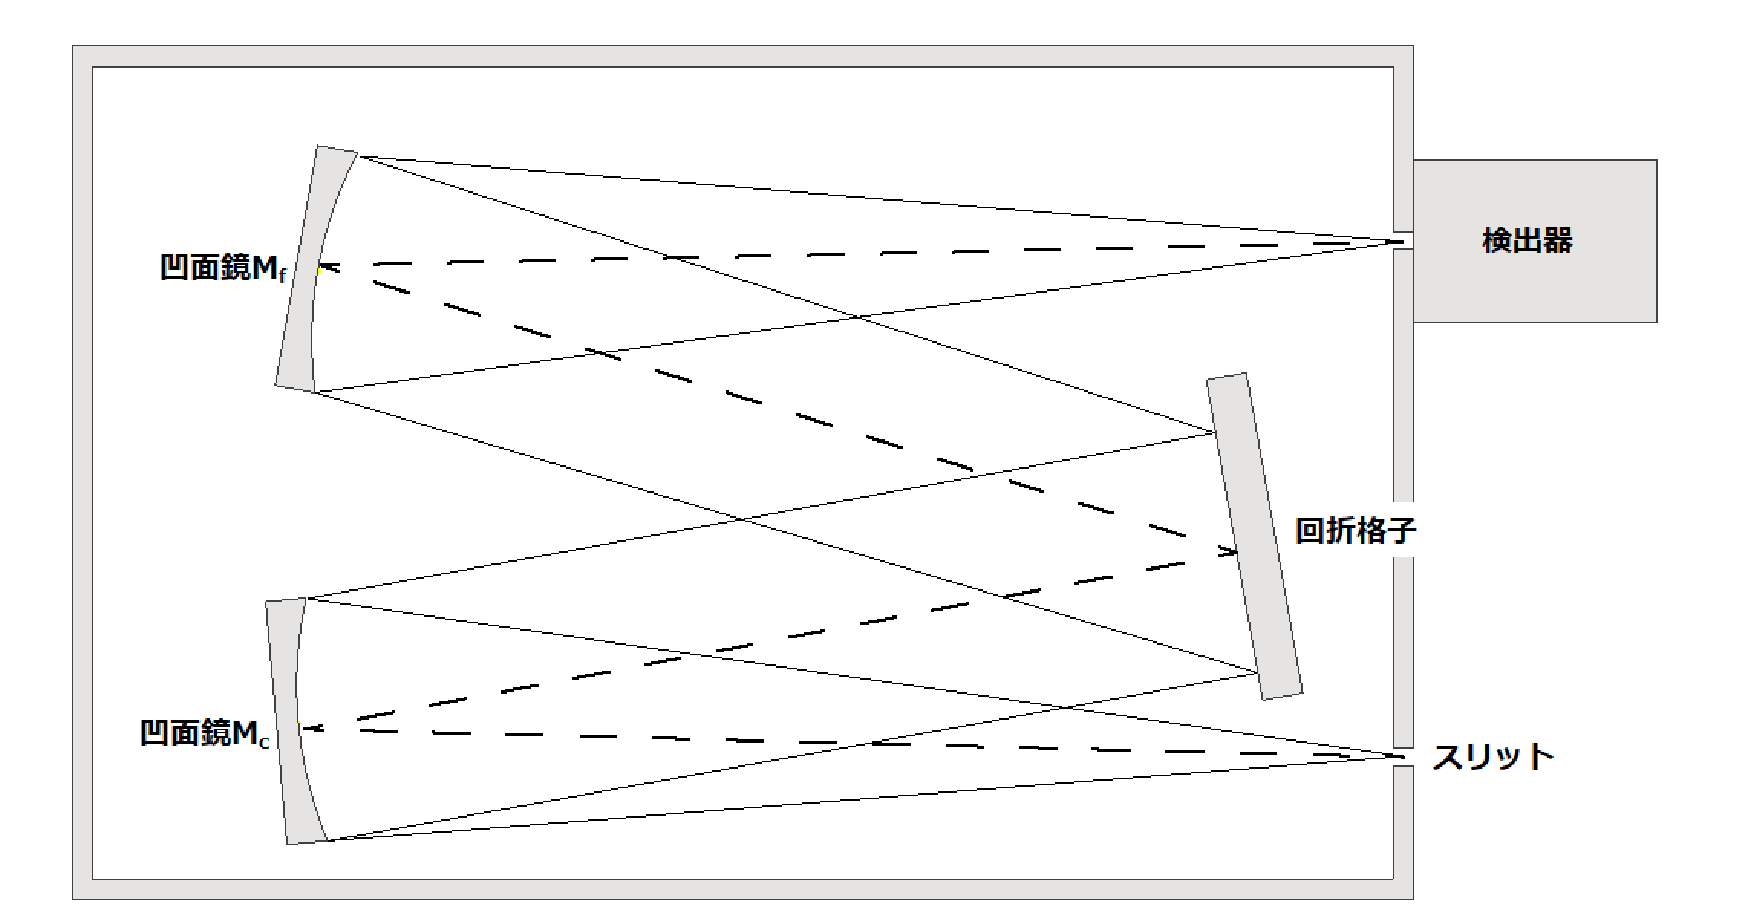
\includegraphics[scale=0.4]{figure/czerny_turner.pdf}
    \caption{ツェルニ・ターナ型分光器の概略図}
    \label{fig:czerny_turner}
\end{figure}
分光器は主にスリット,コリメータ,結像器,回折格子,検出器から構成されている.
ツェルニ・ターナ型分光器ではコリメータ及び結像器には凹面鏡が使用されている.
また,検出器にはCCDカメラやCMOSカメラが用いられている.
この分光器にさまざまな波長の光を入れた場合について考える.
入口スリットから入った光は凹面鏡$\mathrm{M_c}$に反射して平行光となり,回折格子に入射する.
回折格子によって光は波長ごとの異なる角度に回折し,凹面鏡$\mathrm{M_f}$によって検出器受光面に結像される.
この時取り出したい波長以外の光は凹面鏡$\mathrm{M_f}$から外れるか,検出器受光面からずれた位置で集光されている.回折格子の角度を調節することで任意の波長の光を観測することができる\cite{spectrometer}.

% 同じく一般的な分光器であるリトロー型分光器はツェルニ・ターナ型におけるコリメート鏡と結像鏡を共用した構成である.\cite{anritsu}

% 緒言で述べた通りツェルニ・ターナ型分光器は光路内に軸外反射を持つため収差が発生しやすい.
% ここでosloを用いて軸外反射のシミュレーションを行う.
% 軸外反射では特にコマ収差という彗星のように尾を引いてぼやける収差の影響が大きい.
% 球面鏡の軸外反射によってコマ収差が生まれている様子をFig.\ \ref{fig:koma_syuusa}に示す.
% \begin{figure}[htbp]
    % \centering
    % 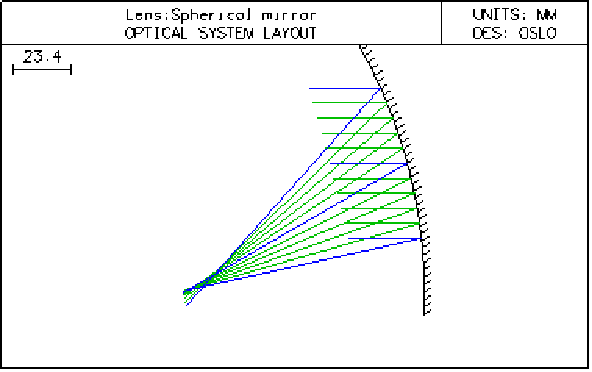
\includegraphics[scale=0.8]{figure/koma_syuusa.pdf}
    % \caption{コマ収差の様子}
    % \label{fig:koma_syuusa}
% \end{figure}
% 緒言で述べた通りツェルニ・ターナ型分光器は光路内に軸外反射を持つため収差が発生しやすい.
% また,軸外反射はより大きな角度で反射するほど収差は大きくなる.

% ツェルニ・ターナ型分光器では二つの凹面鏡を近付けるほど軸外反射の角度を小さくすることができる.
% また同様に凹面鏡から回折格子までの距離を離せば離すほど軸外反射の角度を小さくすることができるが,一般に回折格子が回転するための余裕などを考え凹面鏡と回折格子の距離を凹面鏡の焦点距離の7~8割程度にして配置しているものが多い.
% 例として有効径が100 mm,焦点距離が約1500 mmの球面鏡を用いて球面鏡から回折格子までの距離を焦点距離の8割である1200 mmにすると,二つの球面鏡を可能な限り近づけて配置しても軸外反射の角度は計算上3.6°となる.
% 実際には二つの球面鏡は少し離れて設置されるので軸外反射の角度は4°ほどになると考えられる.


% ここで高度な光線追跡やスポットサイズ解析などを行えるソフトウェアであるOSLOを用いて軸外反射のシミュレーションを行う.
% 球面鏡を結像器として用いた際のスポットの様子を作成した.
% Fig.\ \ref{fig:off_axis_spot_0},Fig.\ \ref{fig:off_axis_spot_1},Fig.\ \ref{fig:off_axis_spot_2}はそれぞれ有効径が100 mm,焦点距離が約1500 mmの球面鏡に対して波長587.6 nmの光を垂直に入射させた際のスポット,軸外反射の角度を2°に設定した際のスポット,軸外反射の角度を4°に設定した際のスポットを表す.
% \begin{figure}[htbp]
%     \centering
%     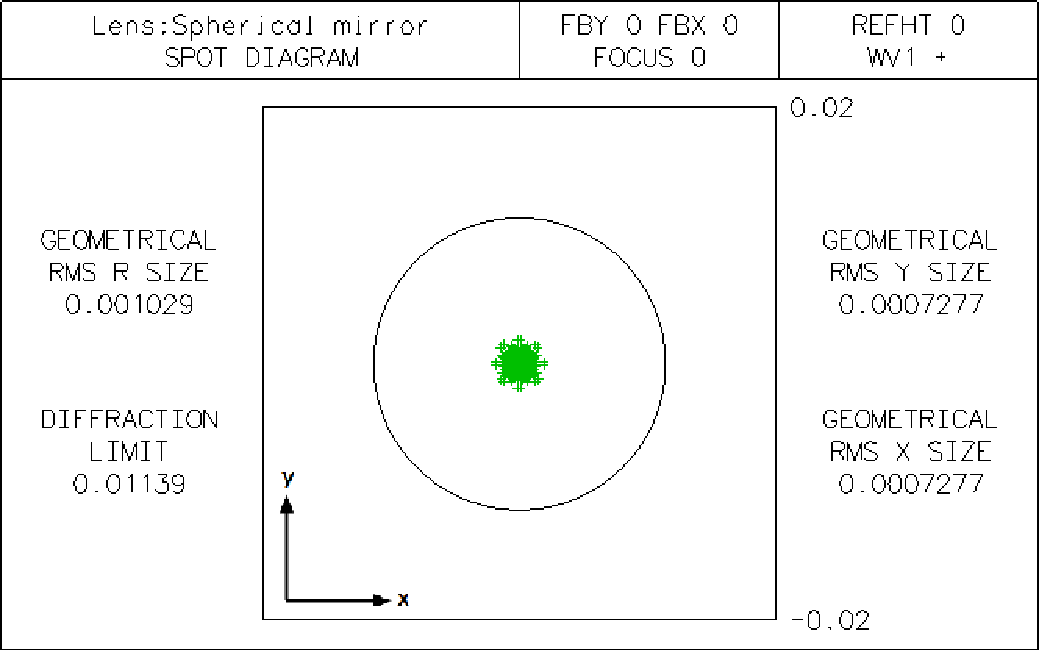
\includegraphics[scale=0.8]{figure/off_axis_spot_0.pdf}
%     \caption{球面鏡で集光した際のスポット(光を垂直に入射)}
%     \label{fig:off_axis_spot_0}
% \end{figure}
% \begin{figure}[htbp]
%     \centering
%     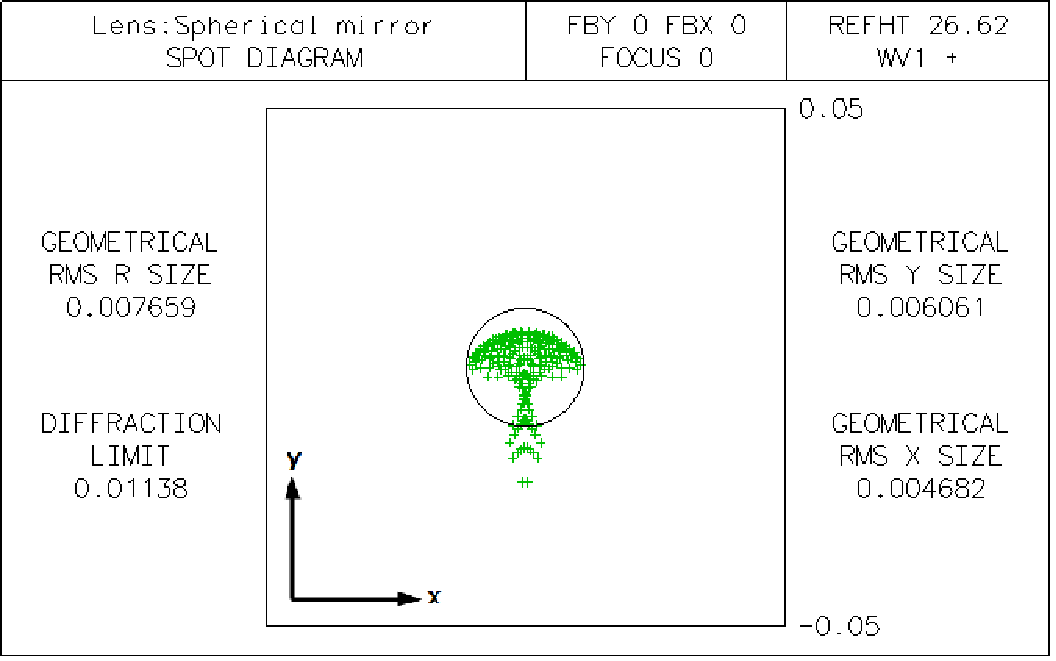
\includegraphics[scale=0.8]{figure/off_axis_spot_1.pdf}
%     \caption{球面鏡で集光した際のスポット(軸外反射の角度を2°に設定)}
%     \label{fig:off_axis_spot_1}
% \end{figure}
% \begin{figure}[htbp]
    % \centering
    % 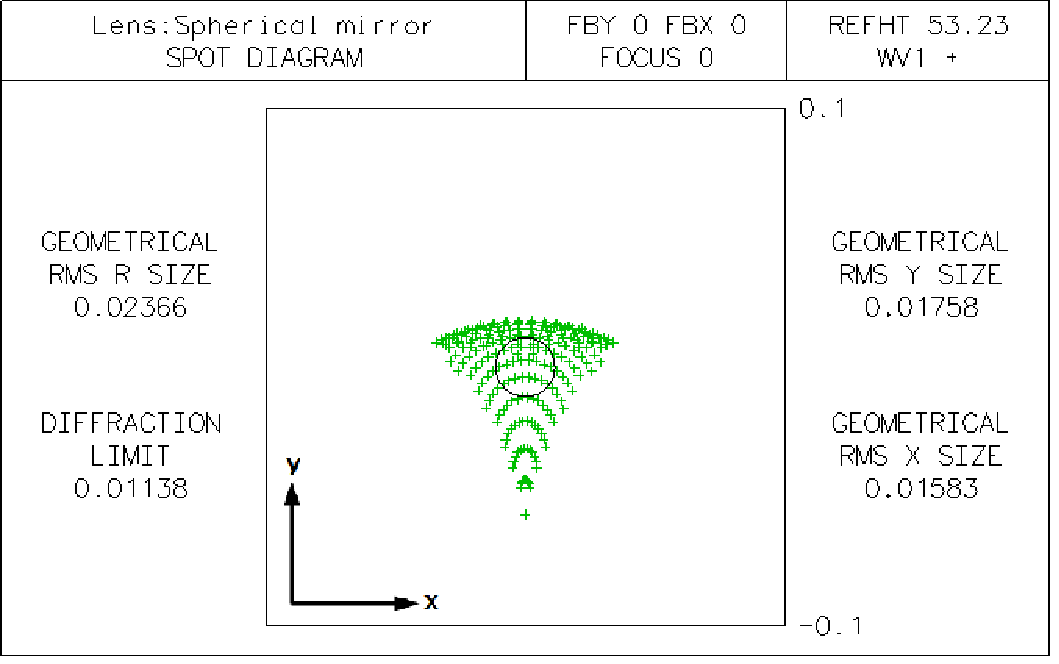
\includegraphics[scale=0.8]{figure/off_axis_spot_2.pdf}
    % \caption{球面鏡で集光した際のスポット(軸外反射の角度を4°に設定)}
    % \label{fig:off_axis_spot_2}
% \end{figure}
% 表示されている数字の単位は全て[mm]である.
% これらの図を見ると軸外反射の角度を大きくするほどスポットが大きくなることがよくわかる.
% 黒い円はエアリーディスクを表しており,Fig.\ \ref{fig:off_axis_spot_0}のようにすべての光線がこの中に収まっている時,回折限界に到達していると言える.
% 対してFig.\ \ref{fig:off_axis_spot_2}のように軸外反射の角度を4°に設定し集光した場合,光はエアリーディスクから大きくはみ出しており,収差の影響を受けることが分かる.
% https://www.an.shimadzu.co.jp/uv/support/lib/uvtalk/uvtalk3/basic.htm


\section{回折格子の基本式}
今回,回折格子が図\ \ref{fig:czerny_turner}のように分光器内で使用されていることを前提に回折格子の基本式について説明を行う.
図\ \ref{fig:grating_principle}に反射型の回折格子による光の回折の様子を模式的に表す.
\begin{figure}[htbp]
    \centering
    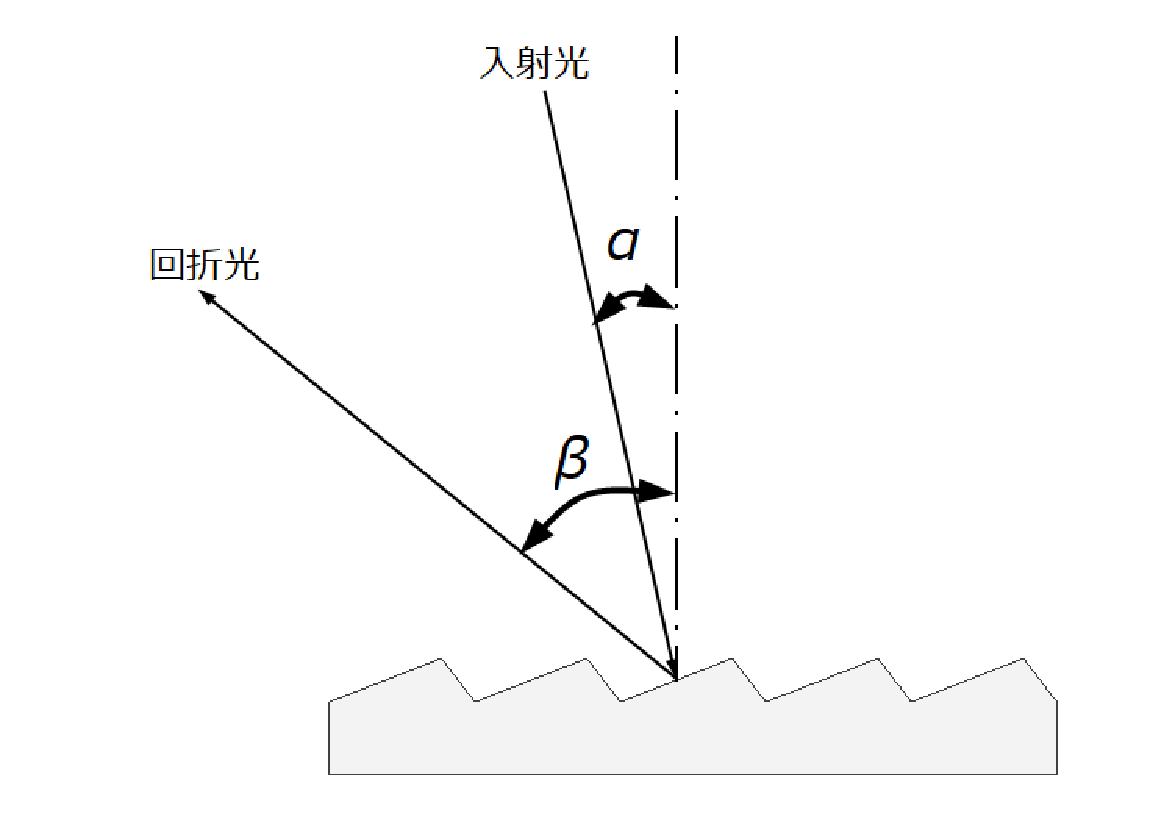
\includegraphics[scale=0.5]{figure/grating_principle.pdf}
    \caption{回折格子における光の回折}
    \label{fig:grating_principle}
\end{figure}
単位長さ当たりの刻線数が$N$の回折格子に波長$\lambda$の光が入射するとき,入射角を$\alpha$,回折角を$\beta$,回折の次数を$m$とすると入射光が回折格子の刻線に垂直な面上にある場合,回折格子の入射角と反射角の関係は以下の式で表される.
\begin{equation}
     Nm\lambda = \mathrm{sin}{\alpha}+\mathrm{sin}{\beta}
\end{equation}
% ここでFig.\ \ref{fig:grating_principle}に示すように入射角と回折角のなす角が$2a$で一定であるとすると,入射角$\alpha$と回折角$\beta$は以下のように表すことができる.
% \begin{eqnarray}
%      \alpha&=&\Phi - a \\
%      \beta&=&\Phi + a
% \end{eqnarray}
% 従って,式(2.1)は
% \begin{eqnarray}
%      Nm\lambda&=&\mathrm{sin}{\alpha}+\mathrm{sin}{\beta} \\
%       &=&2\mathrm{sin}{\frac{\alpha+\beta}{2}}\mathrm{cos}{\frac{\alpha-\beta}{2}}\\
%       &=&2\mathrm{sin}{\Phi}\mathrm{cos}{a}
% \end{eqnarray}
% とできる.
% ここで,$\Phi$は入射角と回折角の二等分線と回折格子の法線がなす角を表す.
% 分光器では$\Phi$を変化させることによって任意の波長を観測することができる.
% レイリーの基準によると,波長$\lambda$のスペクトルの第1極小値の位置に$\lambda+	d\lambda$のスペクトルの最大値がくるときを波長分解の限界と定義している.
% このときの分解能$\lambda/	d\lambda$を理論分解能といい次式で表される.
% \begin{equation}
    %  \frac{\lambda}{d\lambda} = m N W
% \end{equation}
% ここで$W$は回折格子の有効幅であり,$NW$は回折格子に光が当たっている部分の総刻線数を表す.
式(2.1)の両辺を$\lambda$で微分すると,回折格子の角分散($d\beta$/$d\lambda$)が得られる.
なお,角分散は波長に対する回折角の変化量を表す.
\begin{eqnarray}
    \frac{d\beta}{d\lambda} = \frac{Nm}{\mathrm{cos}{\beta}}
\end{eqnarray}
逆線分散は検出器結像面上において単位長さ離れた位置での波長差を表す.
結像器の焦点距離を$f$として,回折角が$d\beta$だけ変化したとき,結像位置が$dx=fd\beta$ずれることから,逆線分散($d\lambda$/$dx$)は次式で表される.
\begin{eqnarray}
    \frac{d\lambda}{dx} = \frac{\mathrm{cos}{\beta}}{Nmf}
\end{eqnarray}
この逆線分散に検出器の受光面の長さを掛けると一度に測定できる波長範囲になる.

回折光の拡大率は分光器において検出器受光面に入射スリットの像が結像される際の像の大きさの倍率を表す.
拡大率($d\alpha$/$d\beta$)は式(2.1)で$\lambda$を一定と置き,両辺を$\beta$で微分すると得られる.
\begin{eqnarray}
    \frac{d\alpha}{d\beta} = -\frac{\mathrm{cos}{\beta}}{\mathrm{cos}{\alpha}}
\end{eqnarray}
スリット幅に拡大率の絶対値($|d\alpha$/$d\beta|$)と逆線分散($d\lambda$/$dx$)を掛け合わせると,スリット幅が有限であることに起因するスペクトルの波長幅になる.
スリット幅を$s$としたとき,この波長幅($d\lambda$)は
\begin{eqnarray}
     d\lambda &=& s\left|\frac{d\alpha}{d\beta}\right|\frac{d\lambda}{dx} \nonumber \\%
        &=&s\frac{\mathrm{cos}{\beta}}{\mathrm{cos}{\alpha}}\frac{\mathrm{cos}{\beta}}{Nmf} \nonumber \\
        &=&\frac{s\mathrm{cos}^2{\beta}}{Nmf\mathrm{cos}{\alpha}}
\end{eqnarray}
と表される.

\section{CCDカメラ}
\subsection{動作原理}
% CCDカメラとはCCDイメージセンサという半導体素子が搭載された高感度のカメラである.
% CCDイメージセンサは光の強さに応じた電荷を出し,電気信号に変換する.
CCDとはCharge Coupled Deviceの略であり,日本語では電荷結合素子と表される光の強さを電気信号に変換する半導体素子である.
CCDは格子状に並んだピクセルから構成されている.
各ピクセルの受光部(フォトダイオード)に光が当たると光の強さに応じた電荷が発生し蓄積される\cite{ccd}.
ここで蓄積された電荷を1ピクセルずつ順次転送して最終的に各画素の電荷を電荷電圧変換アンプで電圧に変換して読み取る\cite{ccd_principle}.
% CCDは光の強さに応じた電荷を出し,その電荷を次々と転送することによって電気信号に変換する半導体のことである.

% CCDにおける電荷転送はよくバケツリレーに例えられるように各ピクセルの持っている信号電荷を隣のピクセルに移すという動作を繰り返すことによって成り立っている.
% 端まで転送された信号電荷は順に電気信号として出力される\cite{ccd}.
% https://www.hamamatsu.com/resources/pdf/ssd/ccd_kmpd9002j.pdf

% https://www.jstage.jst.go.jp/article/itej/68/2/68_145/_pdf

\subsection{ビニング}
CCDでは複数の隣接するピクセルの信号電荷を加算し一つのピクセルとして出力することが可能である.
この動作をビニングと呼ぶ.
ここで,ビニングしたピクセルの数をビニングサイズと呼ぶこととする.
ビニングを行うと解像度が低下する.
一方,ビニングを行うと読み出し回数が減るため読み出しノイズが減少し読み出しスピードが速くなる.
S/N比が良くなるため,微弱な光を読み取る場合にはビニングは有効である.




% https://www.jstage.jst.go.jp/article/lsj/39/10/39_780/_pdf
\chapter{収差と回折限界}
\label{chap:basic_matters}
分光器の分解能は収差と回折限界の影響を受ける.
% 本章では分光器の分解能を考えるうえで大切な要素である収差の評価を行う.
本章では,高度な光線追跡及びスポット解析が行えるソフトウェアであるOSLOを用いて収差と回折限界が分解能に与える影響についてシミュレーションを行う.
スポット解析とはレンズや凹面鏡などで集光した際の結像面での光線の集まり方を調べることである.
この際の結像面での光の分布図をスポット図という.
図\ \ref{fig:OSLO_spot_example}に,OSLOによって作成した光線追跡図及びスポット図の例として焦点距離486.2 mm,有効径100 mmの凸レンズに波長587.6 nmの平行光を入射させた際のシミュレーション結果を示す.
\floatsetup[figure]{style=plain,subcapbesideposition=top}
\begin{figure}
    \sidesubfloat[]{
        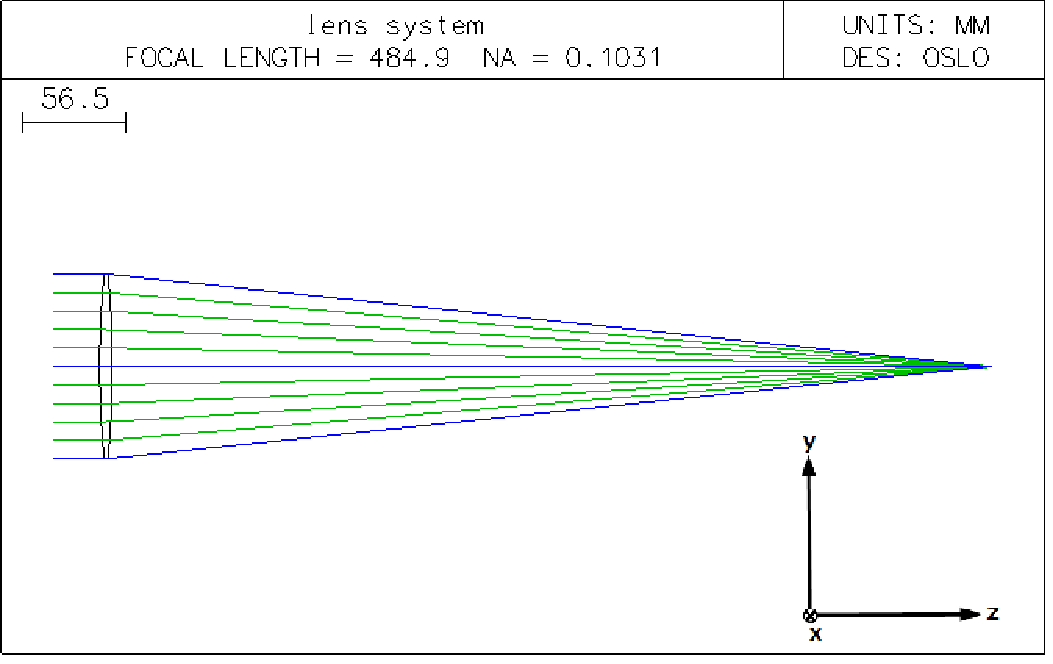
\includegraphics[scale=0.35]{figure/OSLO_raytrace_example.pdf}}
    \sidesubfloat[]{
        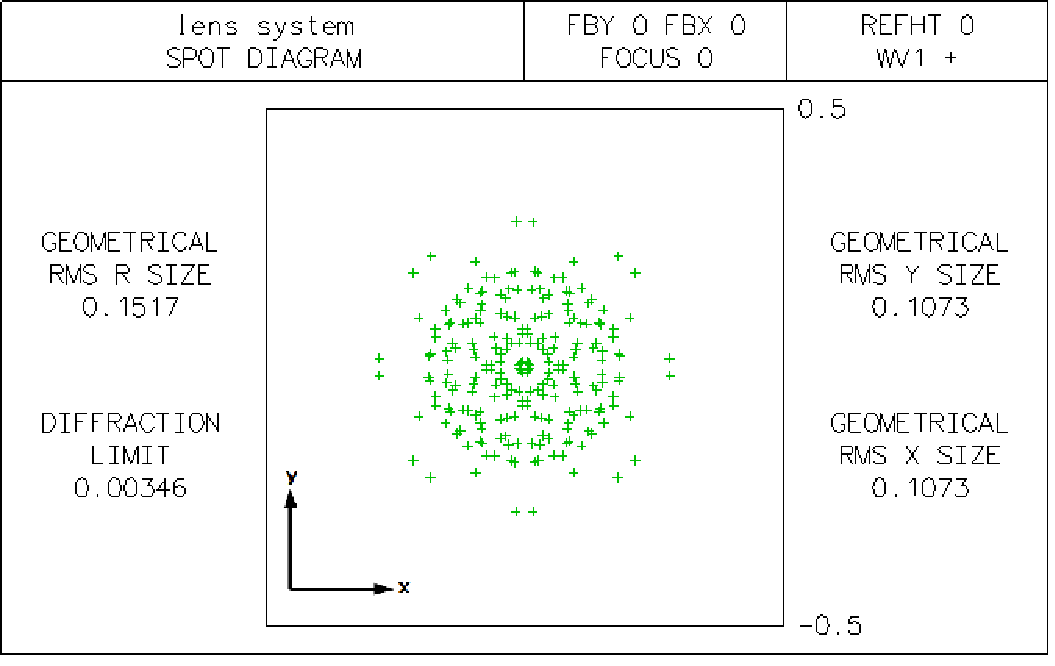
\includegraphics[scale=0.35]{figure/OSLO_spot_example.pdf}}
    \caption{OSLOによるシミュレーションの例(焦点距離486.2 mm,有効径100 mmのレンズを設定) \\
    \centering(a)光線追跡図,
    (b)焦点面でのスポット図}
    \label{fig:OSLO_spot_example}
\end{figure}
ここで,図中にあるように座標系を設定した.
本研究におけるOSLOによるシミュレーションにおいて座標系は図\ \ref{fig:OSLO_spot_example}と同じ設定とし,光は常にz軸負の方向からz軸に平行に入射されるものとする.
図中の数字の単位は全てmmであり,これ以降に出てくる光線追跡図及びスポット図についても同様であるとする.


% ここで,図\  \ref{fig:OSLO_spot_example}(b)のようにある面に対して光を結像させたとき光の分布は二次元のガウス関数で近似できるとすると,スポット図にあるGEOMETRICAL RMS R SIZE($rms_r$と置く)は半径方向の二乗平均平方根であり,ガウス関数の標準偏差$\sigma$に対応する.
% この結像の大きさ$\phi$を光の分布図をガウス関数に近似した際の半値全幅と定義する.
% ガウス関数において半値全幅($FWHM$)は
% \begin{eqnarray}
%      FWHM &=& 2\sigma\sqrt{2\log2} \\
%      &\simeq&2.35\sigma
% \end{eqnarray}
% とできるため,結像の大きさ$\phi$は$2.35rms_r$となる.
% OSLOによるシミュレーションで求められた結像の大きさ$\phi$のことを以下ではスポットサイズと呼ぶこととする.


\section{収差}
レンズや凹面鏡を用いて平行光を集光させる際,一点に結像させるのが理想であるが現実には不可能であり像には歪みやぼけが生じる.
その歪みやぼけのことを収差という.
収差は大きく分けて波長に依存する色収差と,波長に依存しない単色収差に分類できる.
単色収差のなかで特に影響の大きい5つの収差のことをザイデル収差と呼び,球面収差,コマ収差,非点収差,像面湾曲,歪曲収差がある.
ザイデル収差の中で同軸に光が入射した際でも発生するものは球面収差のみで,他の収差は非同軸系で発生する軸外収差である\cite{syuusa}.

\subsection{色収差}
% 色収差はレンズ特有のものである.
% レンズの媒質であるガラスなどの屈折率が波長によって変化することから生まれる焦点距離のずれのことである.
色収差とは波長にとって物質の屈折率が異なるために発生する焦点距離のずれのことである.
そのため,光を反射することで集光を行なっている凹面鏡では色収差は存在しない.
対して,レンズには色収差があり白色光を入射すると,波長の短い青色光の焦点が波長の長い赤色光の焦点よりも短くなる.
そのためレンズに白色光を入射させたとき結像面において色のにじみが発生する\cite{irosyuusa}.

% https://www.jstage.jst.go.jp/article/jpnjvissci/29/1/29_29.3/_pdf/-char/en


\subsection{球面収差}
球面収差とはレンズや凹面鏡の面が球面であることによって生じる収差のことである.
ここではレンズに平行光を入射させたときを例に球面収差の説明を行う.
図\ \ref{fig:kyuumensyuusa_example}に焦点距離が29.7 mm,有効径が20 mmのレンズに波長587.6 nmの平行光を入射させるときの光線追跡図を示す.
\begin{figure}[htbp]
    \centering
    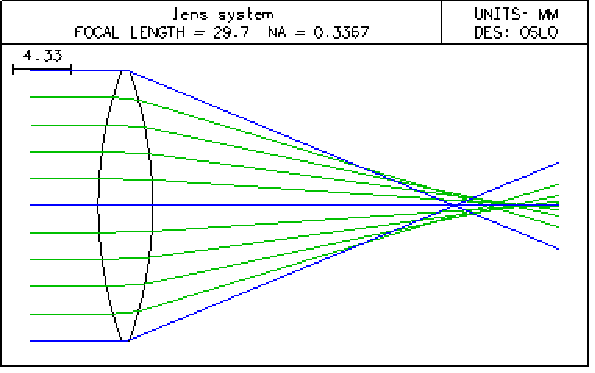
\includegraphics[scale=0.8]{figure/kyuumensyuusa_example.pdf}
    \caption{球面収差が発生している様子}
    \label{fig:kyuumensyuusa_example}
\end{figure}
レンズに入射する各光線で光軸からの距離が大きい光線ほどレンズ面に対する入射角が大きくなり光の屈折が大きくなる.
その結果,入射光線が光軸から離れるほどレンズ近くで焦点を持つ.
これによりレンズの光軸近くに入射する光と光軸から離れた所に入射する光で焦点の位置に差が生じる.



\subsection{コマ収差}
% コマ収差とは彗星のように尾を引いてぼやける収差のことである.
コマ収差はレンズや凹面鏡に対して斜めに光が入射することによって生じる収差である.
コマ収差が発生している様子の例として図\ \ref{fig:koma_syuusa}に焦点距離が100 mm,有効径が30 mmの凹面鏡で波長587.6 nmの平行光を軸外反射によって光軸を30°曲げて集光している様子を示す.
\floatsetup[figure]{style=plain,subcapbesideposition=top}
\begin{figure}
    \sidesubfloat[]{
        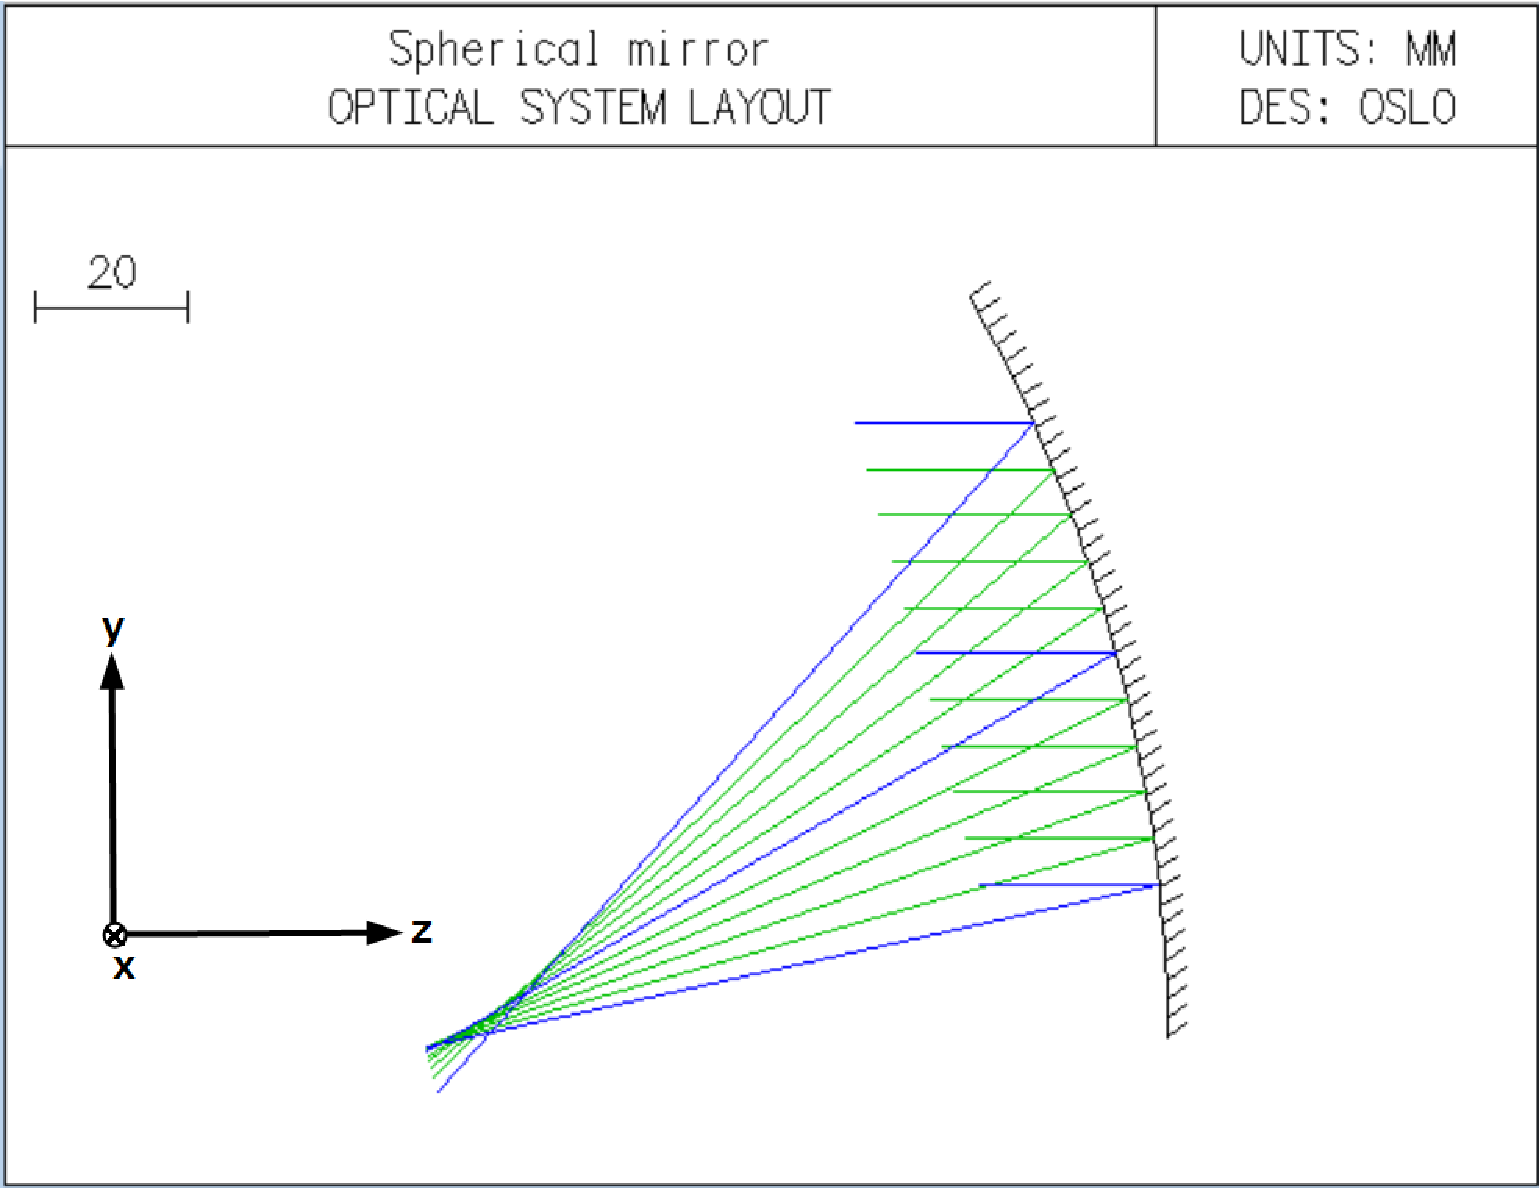
\includegraphics[scale=0.2]{figure/koma_syuusa_zahyou.pdf}}
    \sidesubfloat[]{
        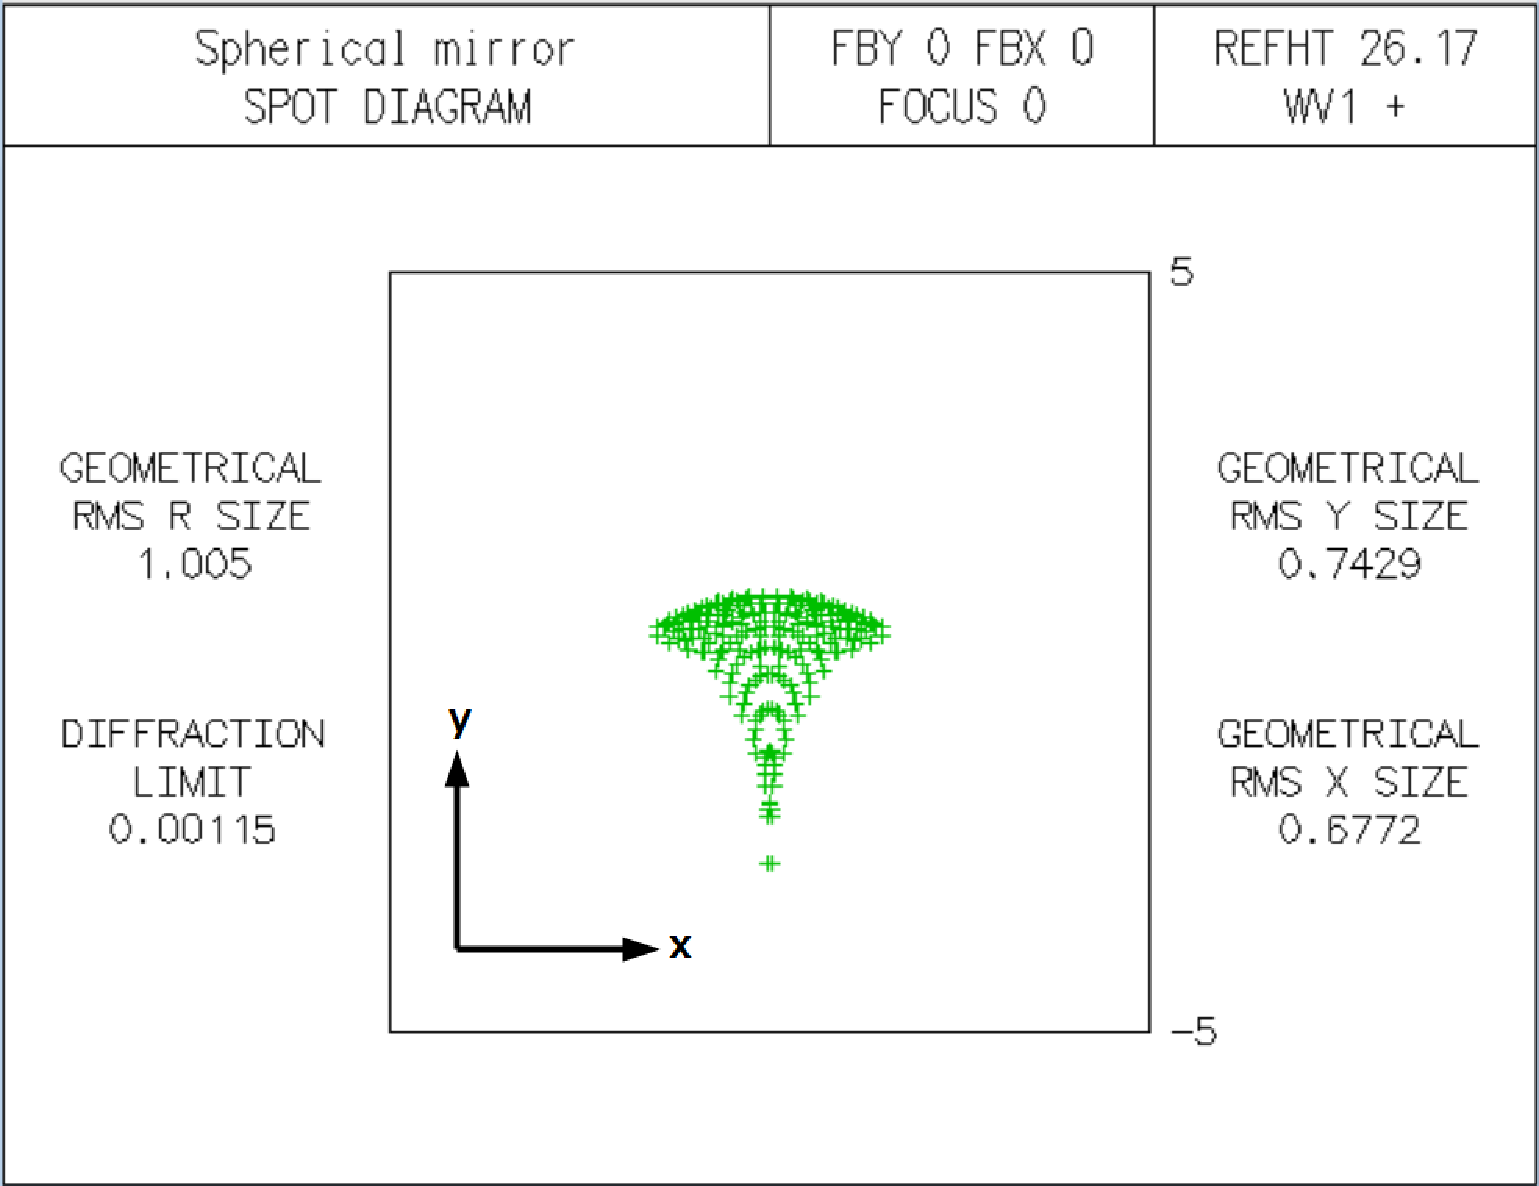
\includegraphics[scale=0.2]{figure/koma_syuusa_spot_zahyou.pdf}}
    \caption{コマ収差が発生している様子 \\
    (a)光線追跡図,
    (b)焦点面でのスポット図}
    \label{fig:koma_syuusa}
\end{figure}
図\ \ref{fig:koma_syuusa}(a)はこのときの光線追跡図を,図\ \ref{fig:koma_syuusa}(b)は焦点面でのスポット図を表す.
% 図\ \ref{fig:koma_syuusa}(a)を見ると主光線(中心を通る光線)に対して光線が非対称になり,結像面において非対称な像を作る.
% これがコマ収差である.
% 図\ \ref{fig:koma_syuusa}(b)はこの凹面鏡において焦点面のスポット図である.
図\ \ref{fig:koma_syuusa}(b)より像がy軸方向に対して非対称になっていることが分かる.
% これがコマ収差である.
図のような彗星のように尾を引いてぼやけることがコマ収差の特徴である.

\subsection{非点収差}
非点収差とは焦点の合う位置の前後で結像の形(縦横比)が変わってぼける収差である\cite{syuusa}.
ここで焦点距離が1525 mm,有効径が98 mmの凹面鏡に対して波長587.6 nmの光を軸外反射によって4°曲げて集光した際,焦点面からz軸方向に+1 mmずらした面でのスポット図及び焦点面からz軸方向に-1 mmずらした面でのスポット図を図\ \ref{fig:hitensyuusa}(a)(b)に示す.
\floatsetup[figure]{style=plain,subcapbesideposition=top}
\begin{figure}
    \sidesubfloat[]{
        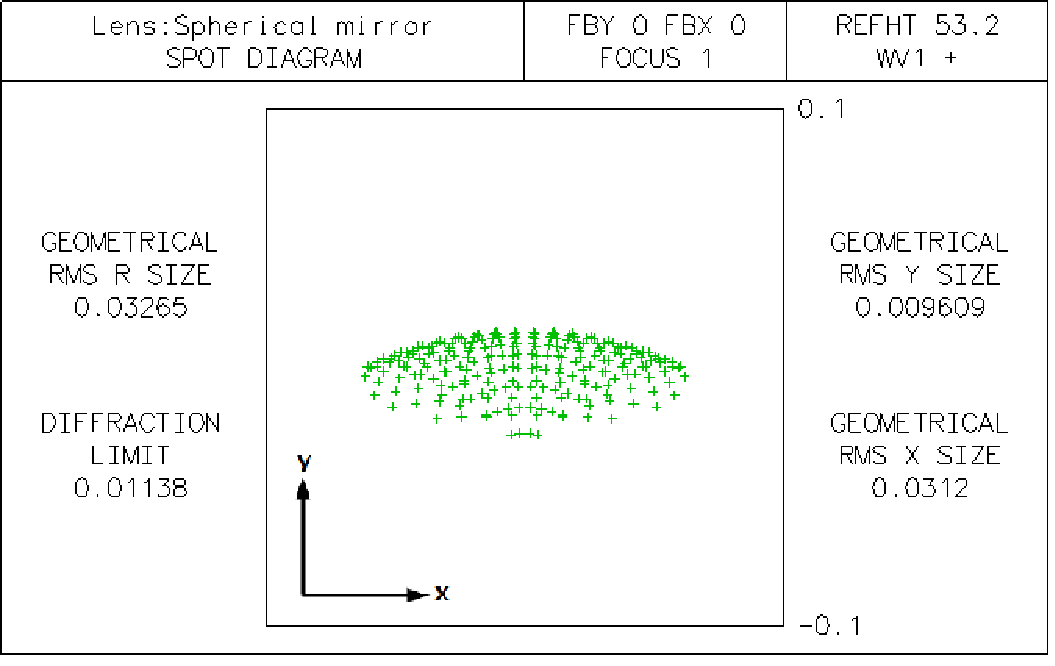
\includegraphics[scale=0.35]{figure/hitensyuusa_1mm.pdf}}
    \sidesubfloat[]{
        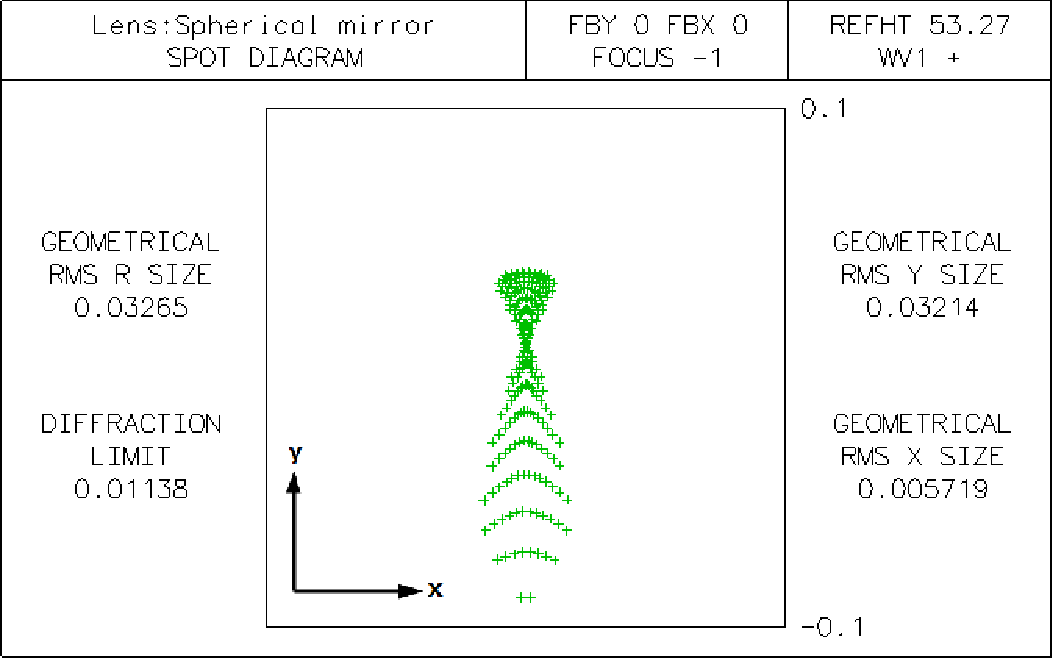
\includegraphics[scale=0.35]{figure/hitensyuusa_-1mm.pdf}}
    \caption[非点収差の様子]{非点収差の様子.焦点距離が1525 mm,有効径が98 mmの凹面鏡で光を軸外反射によって4°曲げて集光した際の焦点面前後のスポット形の変化を表す.\\
    (a)焦点面からz軸方向に+1 mmずらした面でのスポット図,
    (b)焦点面からz軸方向に-1 mmずらした面でのスポット図}
    \label{fig:hitensyuusa}
\end{figure}
図を見るとz軸方向に+1 mmずらした面ではx軸方向に長く結像されているのに対し,z軸方向に-1 mmずらした面ではy軸方向に長く結像されており,焦点前後でぼけ方が変わっていることが分かる.
これは主光線を含むyz平面(子午面)と子午面に垂直なxz平面(球欠平面)内の光線の焦点距離が異なるために発生する.

\subsection{像面湾曲・歪曲収差}
像面湾曲とは,平面から出た光が曲面に結像する収差である.
像面湾曲があると中心で焦点が合っていても周辺で焦点が合わないという現象が起こる.
歪曲収差とは光軸からの距離に応じて像の倍率が異なってくるために起こる歪みのことで,像の形が歪んで見える収差である\cite{nikon}.


% https://www.jstage.jst.go.jp/article/jpnjvissci/36/3/36_40/_pdf/-char/ja

\section{回折限界}
どれだけ収差が抑えられたレンズや凹面鏡を用いても光を一点に集光することはできない.
光の波動性のため回折によって広がってしまうためである.
この回折に制限される分解能の限界のことを回折限界という.

回折限界で結像された光の像は中央部に明るい領域を持ち,その周囲に暗い同心円状輪帯を有するエアリーパターンという回折パターンとなる(図\ \ref{fig:Airy_pattern}).
\begin{figure}[htbp]
    \centering
    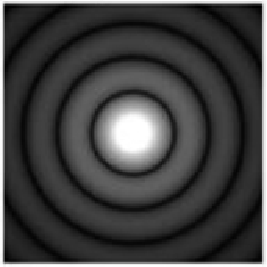
\includegraphics[scale=1.0]{figure/Airy_pattern.pdf}
    \caption{エアリーパターンの模式図\cite{Airy}}
    \label{fig:Airy_pattern}
\end{figure}
中心の明るい領域をエアリーディスクと呼ぶ\cite{airy_disc}.
エアリーディスクの大きさはレンズの焦点における最小の結像サイズである.
エアリーディスクの半径$R$は
\begin{eqnarray}
    R = 1.22\lambda f_{\#}
\end{eqnarray}
と表される.
ここで$\lambda$は光の波長,$f_{\#}$はレンズのf値を表す\cite{airy_disc}.

スペクトルのエアリーディスク部分をガウス関数で近似したときの標準偏差$\sigma$は
\begin{equation}
     \sigma \simeq 0.42\lambda f_{\#}
\end{equation}
と表され\cite{airy_gauss},半値全幅($FWHM$)は
\begin{eqnarray}
     FWHM &=& 2\sigma\sqrt{2\log2} \nonumber \\
     &\simeq&0.99\lambda f_{\#}
\end{eqnarray}
となる.
% https://www.edmundoptics.jp/knowledge-center/application-notes/imaging/limitations-on-resolution-and-contrast-the-airy-disk/




分光器の検出器結像面に回折限界の幅で結像した時が分光器の波長分解の限界である.
その際のスペクトルの波長幅($\delta\lambda$)は逆線分散に先ほどの半値全幅を掛けたものとなる.
ここで,$f_{\#}$はレンズの有効径を$W$とした時$f_{\#}=f/W$であることから
\begin{eqnarray}
     \delta\lambda &=& \frac{\mathrm{cos}{\beta}}{Nmf}\cdot\frac{0.99\lambda f}{W} \nonumber \\
     &=&\frac{0.99 \lambda \mathrm{cos}{\beta} }{mNW}
\end{eqnarray}
とできる.
これが,理論的なスペクトルの最小波長幅である.
% このときの分解能$	d\lambda$を理論分解能といい次式で表される.
% \begin{equation}
    %  d\lambda= \frac{\lambda}{mNW}
% \end{equation}
% ここで$W$は回折格子の有効幅であり,$NW$は回折格子に光が当たっている部分の総刻線数を表す.
% https://www.shimadzu.co.jp/products/opt/guide/05.html




\section{凹面鏡とレンズの結像性能の比較}
本節ではツェルニ・ターナ型分光器のように凹面鏡の軸外反射によって集光・結像する場合と,本実験で採用するアクロマティックレンズを用いて同軸に集光する場合のそれぞれの結像の大きさをOSLOでシミュレーションを行う.
本研究で使用するレンズは焦点距離1525 mm,有効径98 mmのものである.
シミュレーションにおいてレンズと条件を合わせるため,焦点距離を1525 mm,有効径を98 mmの凹面鏡を用いることにした.
また,入射する光は波長587.6 nmの単色光とした.


\subsection{凹面鏡を用いた結像}
ツェルニ・ターナ型分光器で用いられている凹面鏡での集光のシミュレーションを行う.
% 軸外反射での集光はより光軸が大きな角度で曲げられているほど収差は大きくなる.
凹面鏡に平行光を入射し同軸で集光した際の焦点面でのスポット図,軸外反射の角度を2°に設定した際の焦点面でのスポット図,軸外反射の角度を3°に設定した際の焦点面でのスポット図,軸外反射の角度を4°に設定した際の焦点面でのスポット図をそれぞれ図\ \ref{fig:off_axis_spot_0},図\ \ref{fig:off_axis_spot_1},図\ \ref{fig:off_axis_spot_1.5},図\ \ref{fig:off_axis_spot_2}に示す.
\begin{figure}[htbp]
    \centering
    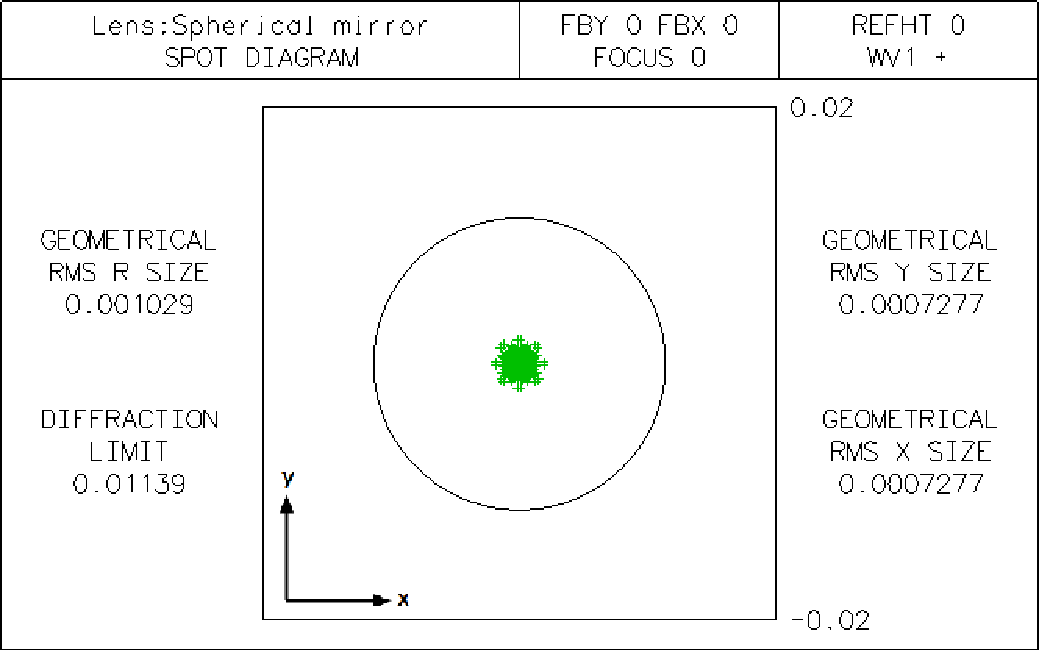
\includegraphics[scale=0.5]{figure/off_axis_spot_0.pdf}
    \caption{凹面鏡で集光した際の焦点面でのスポット図(同軸で集光)}
    \label{fig:off_axis_spot_0}
\end{figure}
\begin{figure}[htbp]
    \centering
    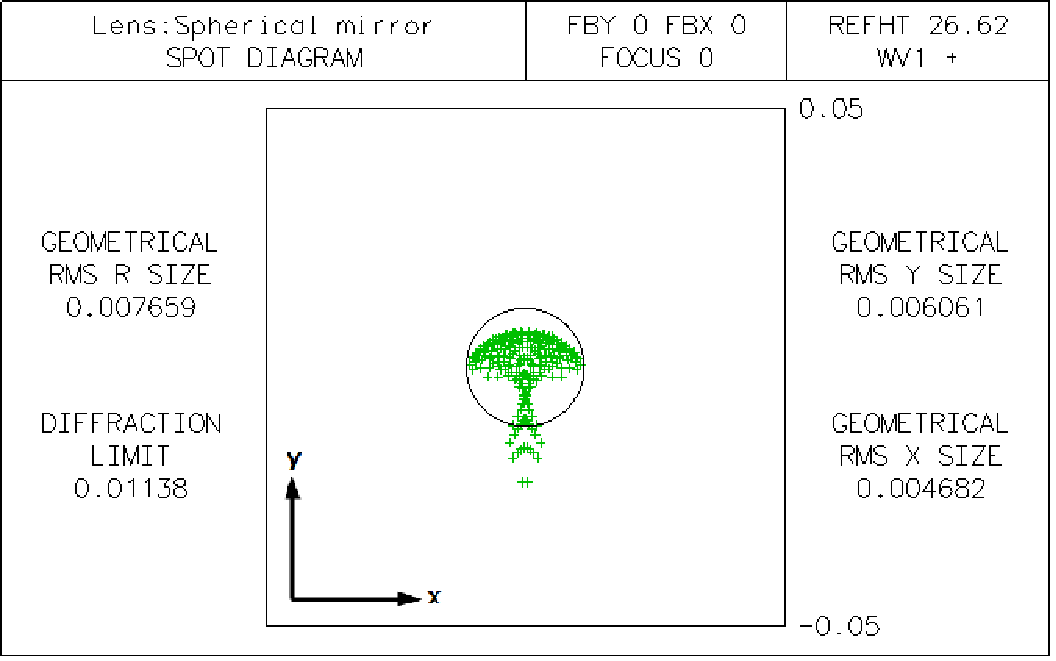
\includegraphics[scale=0.5]{figure/off_axis_spot_1.pdf}
    \caption{凹面鏡で集光した際の焦点面でのスポット図(軸外反射の角度を2°に設定)}
    \label{fig:off_axis_spot_1}
\end{figure}
\begin{figure}[htbp]
    \centering
    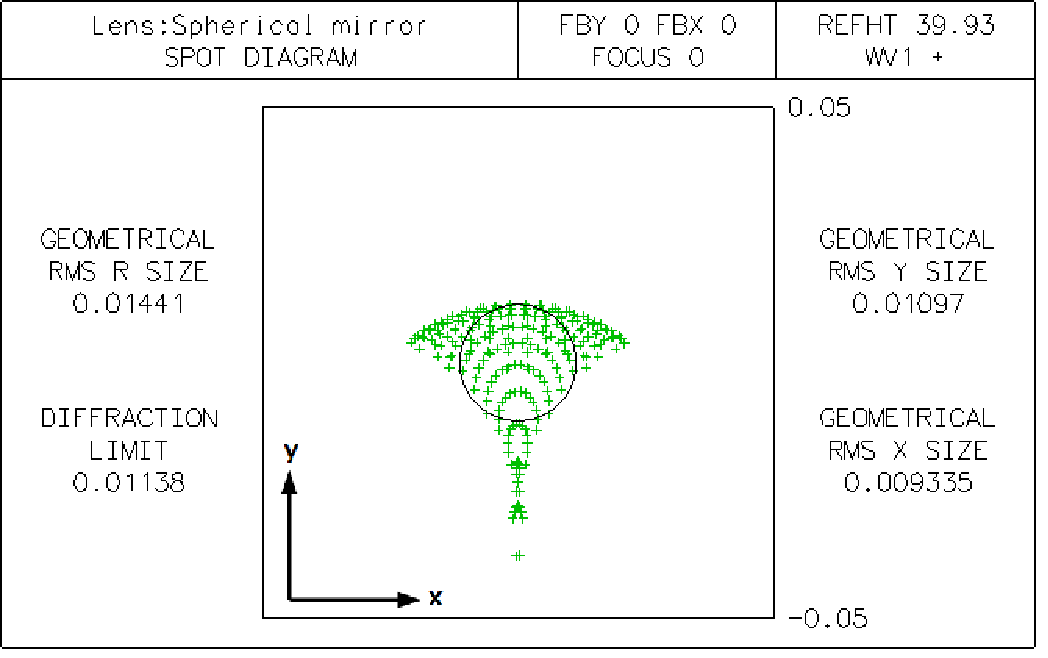
\includegraphics[scale=0.5]{figure/off_axis_spot_1.5.pdf}
    \caption{凹面鏡で集光した際の焦点面でのスポット図(軸外反射の角度を3°に設定)}
    \label{fig:off_axis_spot_1.5}
\end{figure}
\begin{figure}[htbp]
    \centering
    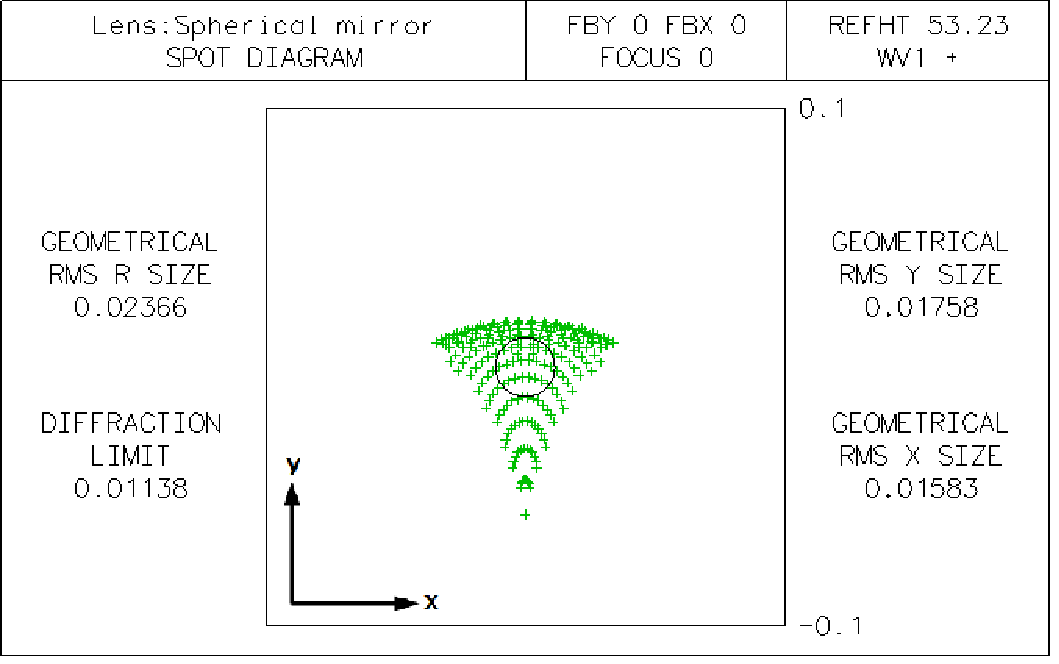
\includegraphics[scale=0.5]{figure/off_axis_spot_2.pdf}
    \caption{凹面鏡で集光した際の焦点面でのスポット図(軸外反射の角度を4°に設定)}
    \label{fig:off_axis_spot_2}
\end{figure}
図中の円はエアリーディスクを表す.
これらの図を見ると軸外反射の角度を大きくするほど結像が大きくなることがよくわかる.
% 同軸で集光した際の結像である図\ \ref{fig:off_axis_spot_0}を見ると全ての光線がエアリーディスク内に集まっているため回折限界で集光できると言える.
% 対して図\ \ref{fig:off_axis_spot_2}のように軸外反射の角度を4°に設定し集光した場合,光はエアリーディスクから大きくはみ出しており,収差の影響を受けることが分かる.

ツェルニ・ターナ型分光器では2つの凹面鏡を近付けるほど軸外反射の角度を小さくすることができる.
また同様に凹面鏡から回折格子までの距離を離せば離すほど軸外反射の角度を小さくすることができるが,一般に回折格子が回転するための余裕などを考え凹面鏡と回折格子の距離を凹面鏡の焦点距離の7~8割程度にして配置しているものが多い.
今回設定した焦点距離を1525 mm,有効径を98 mmの凹面鏡を用いて凹面鏡から回折格子までの距離を焦点距離の8割である1220 mmにすると,二つの凹面鏡を可能な限り近づけて配置しても軸外反射の角度は計算上約2.8°となる.
実際には二つの凹面鏡は少し離れて設置しないと回折格子が光路を遮ってしまうので軸外反射の角度は最小で3°ほどになると考えられる.

図\ \ref{fig:off_axis_spot_1.5}のように軸外反射の角度を3°に設定し集光した場合,光はエアリーディスクからはみ出しており,収差の影響を受けることが分かる.
従って,ツェルニターナ型の分光器の配置では焦点距離が1525 mmと長い凹面鏡を使用しても回折限界での集光は難しく,分解能が収差の影響を受ける.


\subsection{アクロマティックレンズを用いた結像}

次章で述べるように本研究ではコリメータ及び結像器にアクロマティックレンズを使用する.
アクロマティックレンズとは異なる二つのレンズが組み合わされたレンズである.
一般に低屈折率ガラスを用いた正レンズと高屈折率のガラスを用いた負レンズで構成されている.

% アクロマティックレンズの特徴として色収差が補正されているという点がある.
アクロマティックレンズでは構成する2つのレンズが補完しあうことにより,単レンズと比べて色収差を抑えることができる.
図\ \ref{fig:achromaticlense}にアクロマティックレンズが色収差を抑えている様子の簡易図を示す.
\begin{figure}[htbp]
    \centering
    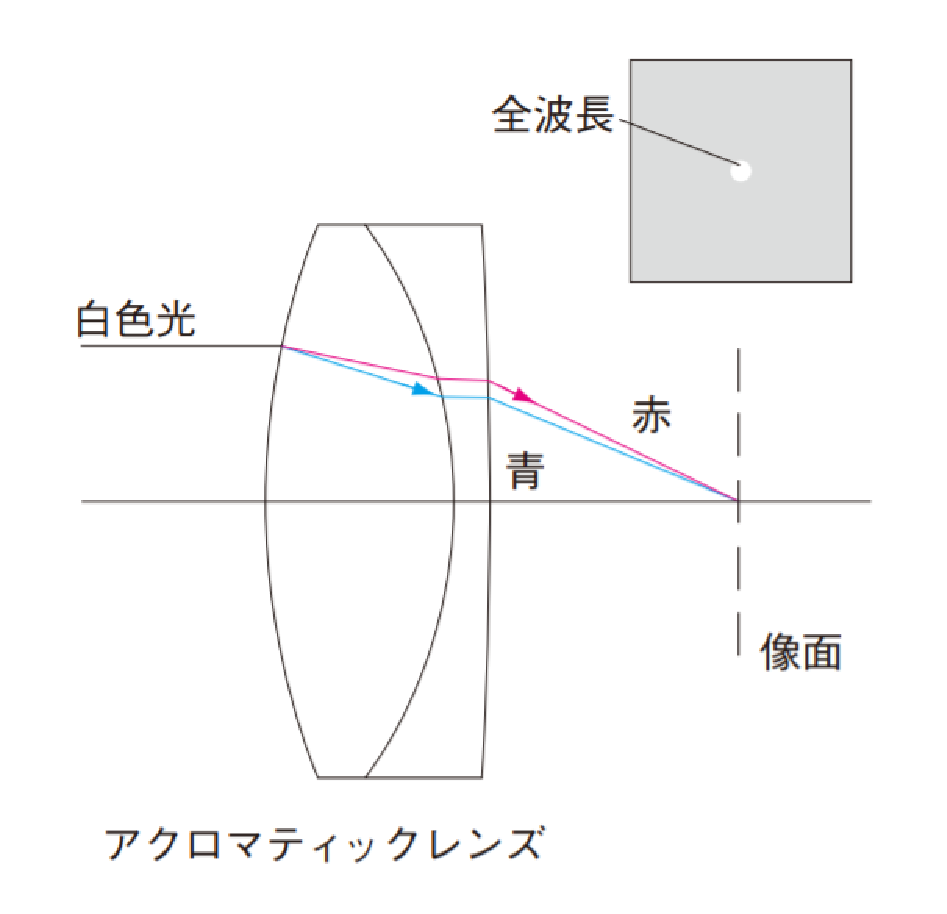
\includegraphics[scale=0.6]{figure/achromaticlense.pdf}
    \caption{アクロマティックレンズでの集光の模式図\cite{achromatic_lens}}
    \label{fig:achromaticlense}
\end{figure}
また,同様に色収差のみでなく球面収差も改善されており,レンズの有効径が大きい場合でも単レンズと比べて小さな結像を得ることができる\cite{achromatic_lens}.


本研究で使用するレンズに平行光を入射させた際の焦点面でのスポット図を図\ \ref{fig:lens_spot}に示す.
\begin{figure}[htbp]
    \centering
    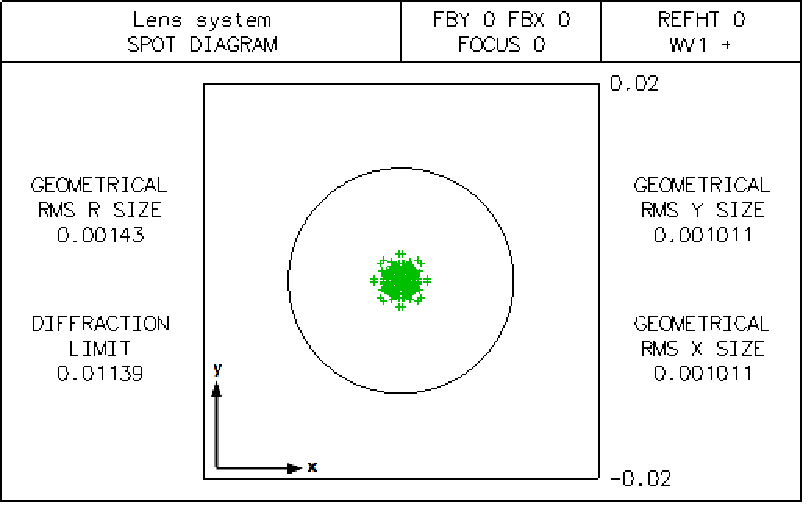
\includegraphics[scale=0.6]{figure/lens_spot.pdf}
    \caption{本分光器の使用レンズで光を同軸に集光した際の焦点面でのスポット図}
    \label{fig:lens_spot}
\end{figure}
全ての光線がエアリーディスク内に集まっているため,回折限界で集光されていると言える.

% 本研究での使用レンズは高い集光性能を持っており,結像面の中心に近いほど光線が多く集まる.
% よって,結像の中心ほど明るくなっている.
結像面における光の分布(光の強度)が二次元のガウス関数で近似できるとすると,スポット図にあるGEOMETRICAL RMS R SIZE($rms_r$と置く)は半径方向の二乗平均平方根であり,ガウス関数の標準偏差$\sigma$に対応する.
この際,結像の大きさ$\phi$を光の分布図をガウス関数に近似した際の半値全幅と定義すると
\begin{eqnarray}
     \phi &=& 2rms_r \sqrt{2\log2} \nonumber \\
     &\simeq&2.35rms_r
\end{eqnarray}
とできる.
以下では,本研究で使用しているレンズの作る設計上の像の大きさをこの$\phi$で定義する.
% \chapter{光学系の構成部品}
本研究ではコリメータ及び結像器にアクロマティックレンズ,検出器にはCCDカメラを用いる.

\section{アクロマティックレンズ}
アクロマティックレンズとは異なる二つのレンズが組み合わされたレンズである.
一般に低屈折率ガラスを用いたの正レンズと高屈折率のガラスを用いた負レンズで構成されている.

アクロマティックレンズの特徴として色収差が補正されているという点がある.
色収差とはガラスの屈折率が波長によって変化することから生まれる焦点距離のずれのことである.
アクロマティックレンズでは構成する二つのレンズが補完しあうことにより,単レンズと比べて色収差を抑えることができる.
Fig.\ \ref{fig:achromaticlense}でアクロマティックレンズが色収差を抑えていることを示す.
\begin{figure}[htbp]
    \centering
    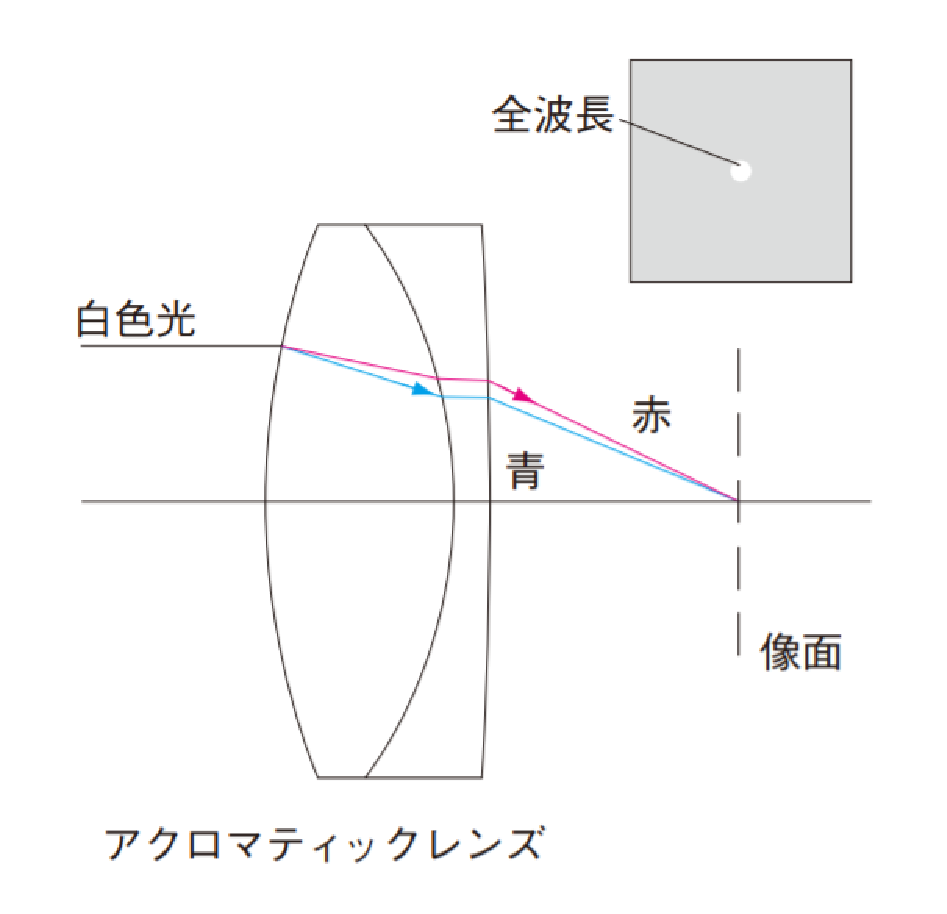
\includegraphics[scale=0.6]{figure/achromaticlense.pdf}
    \caption{アクロマティックレンズでの色収差の補正\cite{achromatic_lens}}
    \label{fig:achromaticlense}
\end{figure}
また,同様に色収差のみでなく球面収差も改善されており,レンズの有効径が大きい場合でも単レンズと比べて小さなスポット径を得ることができる.



% ここで,osloを用いてこのアクロマティックレンズがどのぐらいのスポット径に集光されるのかシミュレーションを行った.



% http://www.mekatoro.net/digianaecatalog/chuo-sougou/book/chuo-sougou-P0904.pdf


\chapter{分光器の設計・製作}
前章で述べた通り,レンズを用いた同軸での集光は凹面鏡での軸外反射による集光と比べ高い集光性能を持つ.
そのため,凹面鏡によって集光する分光器と比べてレンズによって集光する分光器の方がより高い分解能を期待できる.
ただしレンズは色収差を持つため,レンズを用いた分光器では測定波長ごとにレンズの位置を変化させ検出器受光面に焦点を合わせる必要がある.

本研究ではコリメータ及び結像器にアクロマティックレンズ,検出器にはCCDカメラを用いる.
ここでより波長分散を大きくするために焦点距離が1525 mmと長焦点のアクロマティックレンズを使用する.
装置全体の大きさを小さく収めるために光路内に複数の平面ミラーを設置し光軸を折り曲げた設計とした.
設計波長域は400 nm~700 nmとした.

\section{分光器の設計}
\label{sec:spectrometer_design}
% 本研究ではコリメータ及び集光器にアクロマティックレンズ,検出器にはCCDカメラを用いる.
図\ \ref{fig:spectrometer_design}に設計した分光器の概略図を示す.
\begin{figure}[htbp]
    \centering
    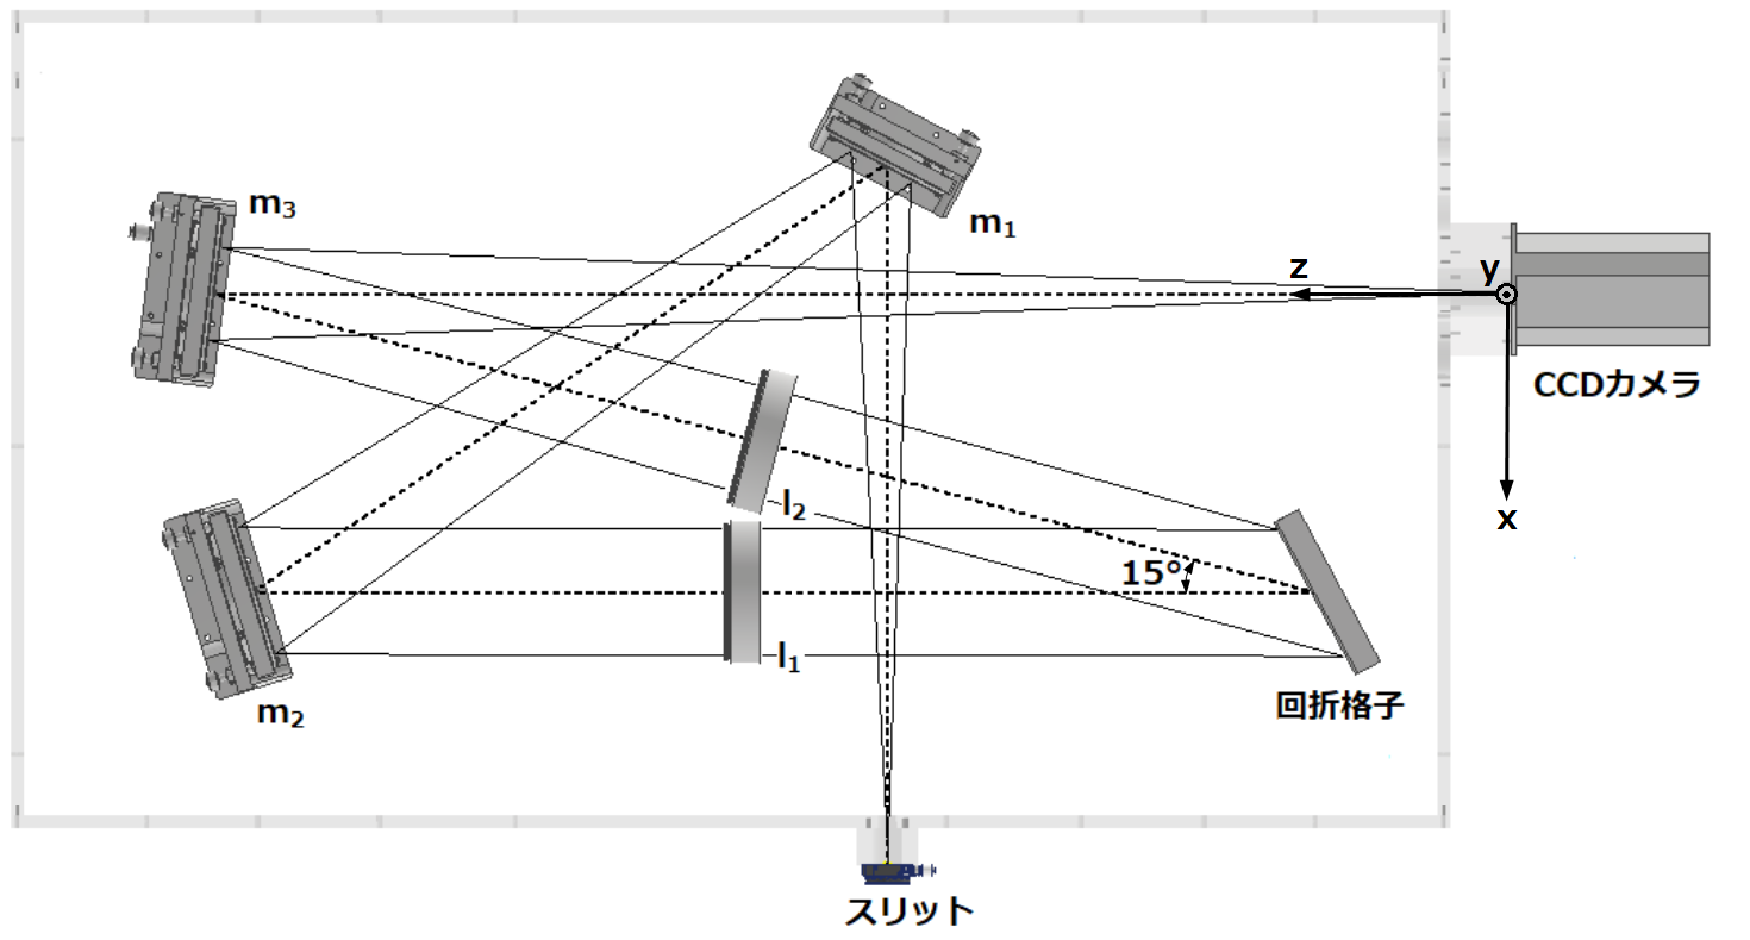
\includegraphics[scale=0.55]{figure/spectrometer_design2.pdf}
    \caption{分光器概略図}
    \label{fig:spectrometer_design}
\end{figure}
入口スリット(スリット幅10 $\mu$m)から入射された光は平面鏡$\mathrm{m_1}$(有効径77 mm)及び平面鏡$\mathrm{m_2}$(有効径96 mm)に反射した後,レンズ$\mathrm{l_1}$(Edmund Optics TS 大口径アクロマティックレンズ $\#$54568,焦点距離1525 mm,有効径98 mm)によって平行光に変えられる.
平行光は回折格子(2400 grooves/mm,$112\times132$ $\mathrm{mm^{2}}$)によって回折される.
その後,レンズ$\mathrm{l_2}$(焦点距離1525 mm,有効径98 mm)を通ることで集光され,平面鏡$\mathrm{m_3}$(有効径96 mm)によって反射された後,検出器であるCCDカメラ(ANDOR DV435,13×13 $\mu\mathrm{m^{2}}$/ピクセル,1024×1024 ピクセル,16 bit)に結像される.
% ここでレンズは球面収差をより抑えるために焦点距離が1525 mmと長いアクロマティックレンズを使用している.
% 装置全体の大きさを小さく収めるために光路内に複数の平面ミラーを設置し光軸を折り曲げた設計とした.
なお,便宜上CCDカメラの受光部の中心を原点に図のように座標系を設定する.

図\ \ref{fig:lens_grating_system}(a)(b)にレンズ及び回折格子周りの各部品の配置を示す.
\floatsetup[figure]{style=plain,subcapbesideposition=top}
\begin{figure}
    \sidesubfloat[]{
        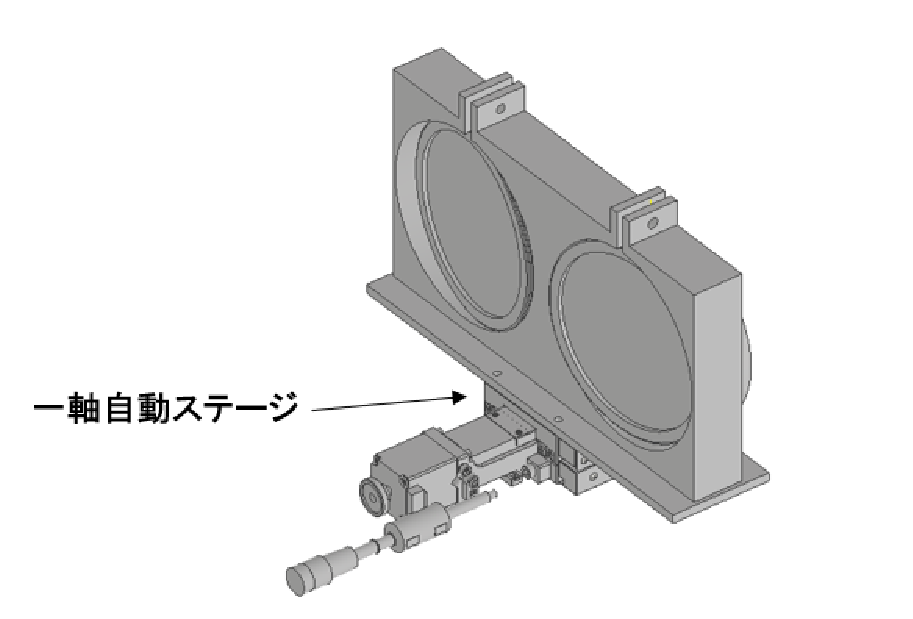
\includegraphics[scale=0.5]{figure/lense_system.pdf}}
    \sidesubfloat[]{
        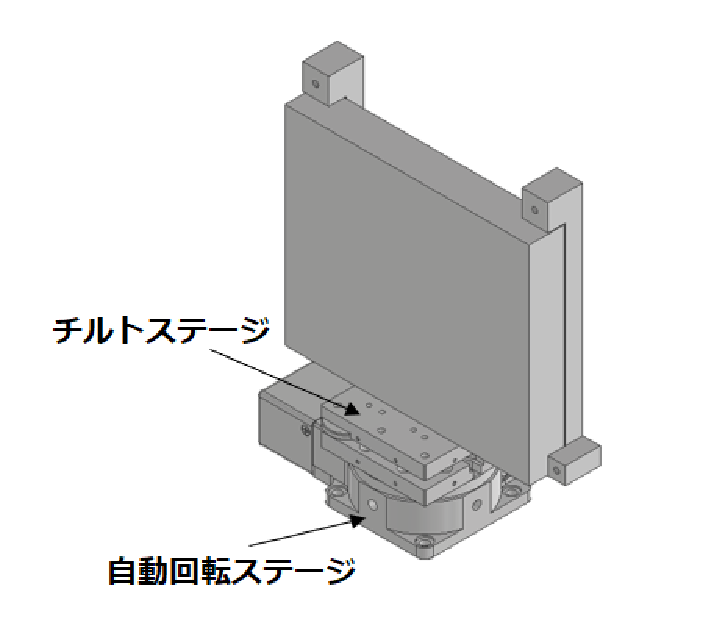
\includegraphics[scale=0.5]{figure/grating_system.pdf}}
    \caption{(a)レンズ周りの部品構成,(b)回折格子周りの部品構成}
    \label{fig:lens_grating_system}
\end{figure}
二つのレンズはレンズホルダによって固定している.
フォーカス調整のためにレンズの下に一軸自動ステージ(シグマ光機株式会社製 HPS60-20X-M5,1 $\mu\mathrm{m}$/パルス,移動量$\pm{10.0}$ mm)を取り付けた.
また,回折格子の下には水平方向の傾きを微調整するためのチルトステージと回折格子の角度(回折格子の面の向き)を制御するための自動回転ステージ(シグマ光機株式会社製 OSMS-60YAW,0.0025°/パルス)を取り付けた.
これらの自動ステージはそれぞれのステージのステッピングモータに入力されるパルス信号で制御されている.
以下では回転ステージ,一軸自動ステージのパルスの絶対値をそれぞれ回折格子パルス,フォーカスパルスと呼ぶこととする.
さらに,レンズ下の一軸自動ステージの移動量が足りない場合を想定して,平面鏡$\mathrm{m_3}$の下には一軸手動ステージ(シグマ光機株式会社製 TSD-601S,移動量$\pm{6.5}$ mm)を取り付けた.
またスリットと分光器筐体の間に取り付けたスリット台の厚みを変えることでスリットのx軸方向の位置を任意に変更できるようにした.

% \floatsetup[figure]{style=plain,subcapbesideposition=top}
% \begin{figure}
%     \sidesubfloat[]{
%         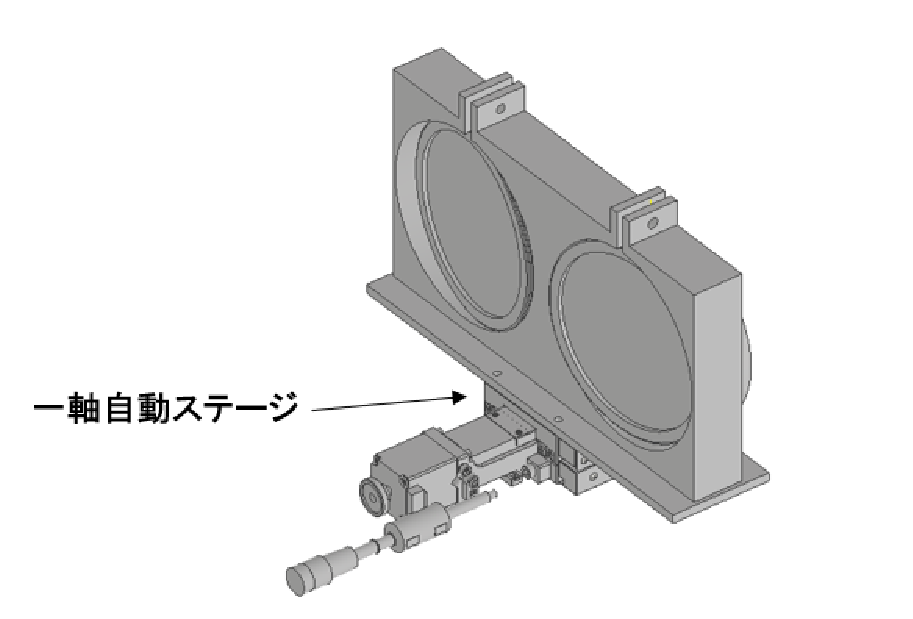
\includegraphics[scale=0.5]{figure/lense_system.pdf}}
%     \sidesubfloat[]{
%         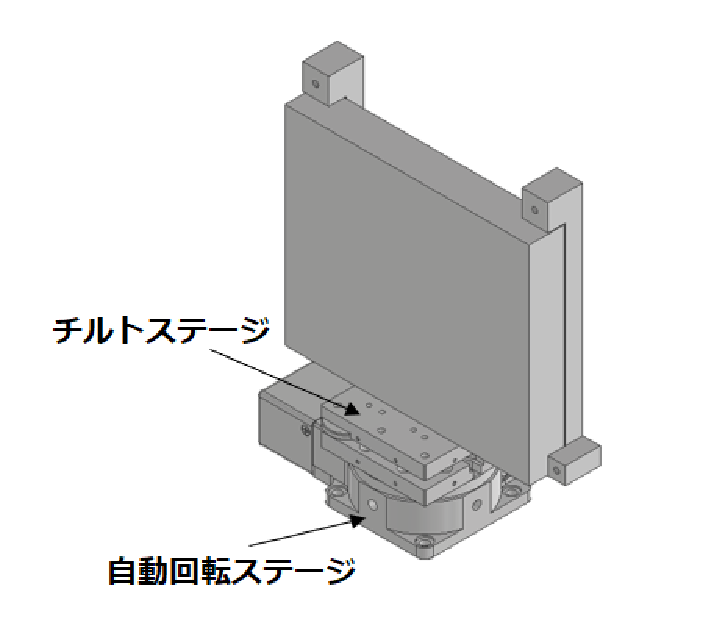
\includegraphics[scale=0.5]{figure/grating_system.pdf}}
%     \captionsetup{
%     (a):レンズ周りの部品構成
%     (b):回折格子周りの部品構成}
%     \label{fig:lense_grating_system}
% \end{figure}

% 本研究では分光器の入口スリットは幅10 $\mu$mのものを使用しているため,CCDカメラの結像面でも10$\mu$mの幅で結像されること期待して設計している.
% それを実現するためには,レンズが直径10$\mu$m以下の大きさに光を結像できる性能を持っている必要がある.
% 使用レンズを用いた際のスポットの様子を確認するためにOSLOを用いてシミュレーションを行った.
% Fig.\ \ref{fig:lens_spot}は今回使用するレンズに波長587.6nmの平行光を入射したときのスポット図を表す.
% \begin{figure}[htbp]
%     \centering
%     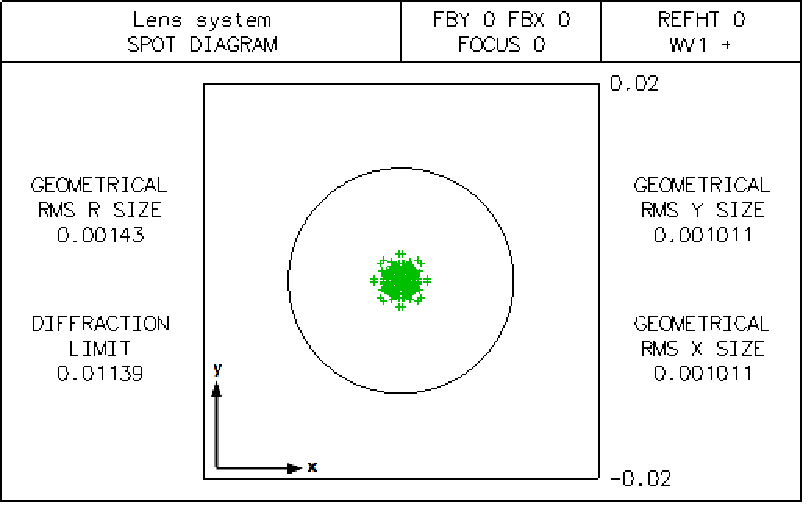
\includegraphics[scale=0.6]{figure/lens_spot.pdf}
%     \caption{波長587.6nmの光を垂直に入射させたときの使用レンズのスポット図}
%     \label{fig:lens_spot}
% \end{figure}
% 全ての光線がエアリーディスク内に収まっており結像の大きさが回折限界によって制限されていることが分かる.

今回二つのレンズを一つのステージでまとめて移動させるように設計したため,各レンズは光軸方向とわずかにずれて移動する.
そのため一軸自動ステージの移動量が大きいほどレンズは光軸から傾く.
一軸自動ステージの移動量の範囲では,最大で約0.16°傾く.

このレンズの傾きによる影響を検証するためにOSLOを用いて結像の様子をシミュレーションした.
レンズに0.16°傾いた光を入射させたときの焦点面でのスポット図を図\ \ref{fig:lens_spot_zure}に示す.
\begin{figure}[htbp]
    \centering
    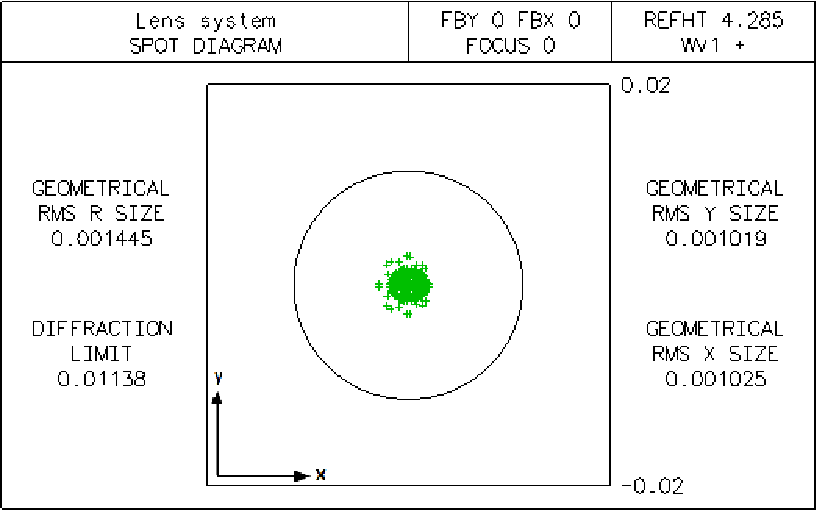
\includegraphics[scale=0.6]{figure/lens_spot_zure.pdf}
    \caption{本分光器の使用レンズに光を0.16°傾けて入射させたとき焦点面でのスポット図}
    \label{fig:lens_spot_zure}
\end{figure}
図から分かるようにすべての光線がエアリーディスク内に収まっていることから0.16°光が傾いて入射しても回折限界で集光できる.
従って,このレンズの傾きによって生まれる収差の影響は小さいと言える.

\section{装置幅の予測}
分光器に単波長の光を入射させたとしても,スペクトルは収差やスリット幅に依存した有限の幅を持つ.
この各分光器ごとに固有であるスペクトルの幅を装置幅と呼ぶ.
設計した分光器の理論的な装置幅を求めるため,設計波長域において装置幅に影響を与えるスリット幅,レンズの収差,回折限界からくる波長幅を比較する.

回折限界における理論的なスペクトルの最小波長幅
\begin{equation}
     \delta\lambda = \frac{0.99 \lambda \mathrm{cos}{\beta} }{mNW}
\end{equation}
及びスリット幅$s$=10 $\mu$mから入った光が理想的に結像された際のスペクトルの波長幅
\begin{eqnarray}
     d\lambda &=& 
        \frac{s\mathrm{cos}^2{\beta}}{Nmf\mathrm{cos}{\alpha}}
\end{eqnarray}
及び使用レンズがつくる設計上の結像の大きさに対応する波長幅を表すものを図\ \ref{fig:instrumental_function_design}に示す.
\begin{figure}[htbp]
    \centering
    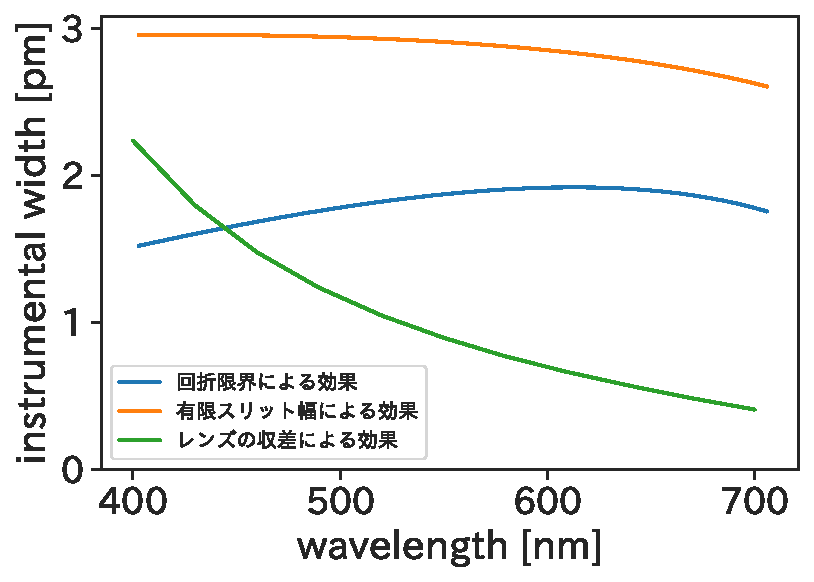
\includegraphics[scale=0.7]{figure/instrumental_function_design.pdf}
    \caption{装置幅に影響を与える要素による波長幅の比較}
    \label{fig:instrumental_function_design}
\end{figure}
% 線1が回折格子の理論分解能,線2が本分光器においてスリット幅の効果で結像されたときの波長幅,線3が使用レンズのスポットサイズに対応する波長幅を表す.
% ここで理想的に結像された際の波長幅とはスリットの幅10 $\mu$mから入射された光が回折格子によって$d\alpha/d\beta$倍に拡大され結像するとした際のスペクトルの波長幅のことでスリット幅s×拡大率の大きさ($|d\alpha/d\beta|$)×逆線分散($d\lambda/dx$)となり以下の式で表される.
% \begin{eqnarray}
%      d\lambda &=& s\left|\frac{d\alpha}{d\beta}\right|\frac{d\lambda}{dx} \\
%         &=&s\frac{\mathrm{cos}{\beta}}{\mathrm{cos}{\alpha}}\frac{\mathrm{cos}{\beta}}{Nmf} \\
%         &=&\frac{s\mathrm{cos}^2{\beta}}{Nmf\mathrm{cos}{\alpha}}
% \end{eqnarray}
使用レンズのつくる設計上の結像の大きさはOSLOを用いて使用レンズに波長400 nmから30 nm間隔で波長700 nmまでの光を入射させた際の焦点面でのスポット図をシミュレーションし,それぞれの$\phi$とした.


図\ref{fig:instrumental_function_design}において回折限界での波長幅及び使用レンズの作る設計上の結像の大きさに対応する波長幅は設計波長域で常にスリット幅10 $\mu$mから入った光が理想的に結像された際の波長幅より小さい.
よって今回の設計において,分光器の装置幅は主にスリット幅によるものであり,レンズの球面収差や回折限界による影響は受けにくいと期待される.


% そこから,本研究では設計波長域においてFig.\ \ref{fig:instrumental_function_design}中の線2に迫る$3.0\times10^{-3}$ nmの装置幅を目指して分光器を製作した.



\section{光学配置の調整}
% 筐体に各部品を取り付けるだけではCCDカメラの受光部に正確に焦点は合わず,各部品の位置・角度の微調整を要する.
% 調整は大きく分けて焦点位置の鉛直方向の調整とフォーカスの調整とがある.



\subsection{結像位置の調整}
xy平面上において結像位置がCCDカメラの受光部からy軸方向にずれていると,いくら回折格子を回転させてもCCDカメラに発光線は映らない.
そこで光源にHeNeレーザー(波長632.8 nm)を用いて,CCDカメラの中心部に結像位置が来るように各ミラー及び回折格子の傾きを調整した.

分光器の設計ではy=0の面に対して対称になるような光学系の配置であるため,回折格子の角度に関係なく結像位置のy座標は全ての発光線において変化しないはずである.
しかし回折格子が水平でなく,入射光と回折格子の刻線に垂直な面に傾きがある場合,対称性が失われ回折格子の角度によって結像位置のy座標は変化してしまう.
そこで今回,回折格子の傾きを直すためHeNeレーザーの$\pm{}$1次光及び0次光の結像位置のy座標の位置を揃えるように調整した.


% これは回折格子の角度によって発光線のy軸方向の結像位置が変化しているということである.
% しかし,今回の分光器の設計ではy=0の面に対して対称になるような光学系の配置であるため,設計通りであればこのような現象は起こりえない.
% 従ってこの現象は回折格子が水平でなく,入射光と回折格子の刻線に垂直な面に傾きあるために生じるものであると考え,それぞれの発光線のy軸方向の位置が揃うようにした.

% そのため,それぞれのスペクトルの高さが揃うようにした.

%  また,平面鏡$m_3$の下の一軸手動ステージを調節しCCDカメラの受光面に焦点が来るように調節を試みた.しかし,一軸手動ステージの移動量では限界があったため,スリットと分光器の筐体の間に3Dプリンタで作成した台を入れることによりさらなる調整を可能にしたd.
\subsection{結像のフォーカス調整}
分光器の分解能を高めるためには発光線をできるだけ細く結像させる必要がある.
従って,レンズの焦点距離にCCDカメラの受光面を正確に合わせるべきである.
結像位置の調整と同じく光源にHeNeレーザーを用いて発光線がCCDカメラ中心になるように回折格子パルスを設定し,フォーカスパルスを等間隔で変化させて31個のデータを撮影した.
図\ \ref{fig:HeNe_focus_example}は撮影した各データにおけるフォーカスパルスとスペクトル幅の関係性を表している.
\floatsetup[figure]{style=plain,subcapbesideposition=top}
\begin{figure}
    \sidesubfloat[]{
        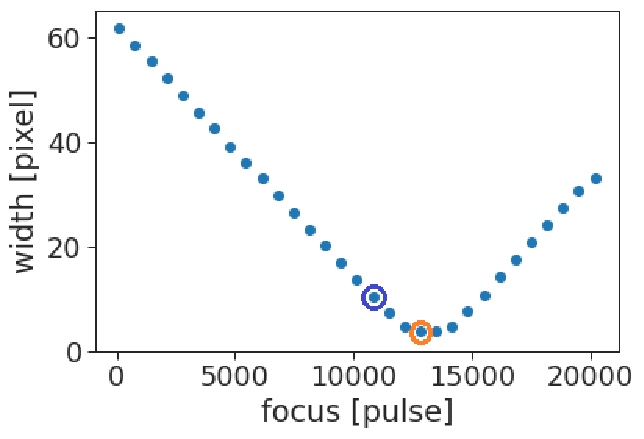
\includegraphics[scale=0.6]{figure/HeNe_focus_example.pdf}}
    \sidesubfloat[]{
        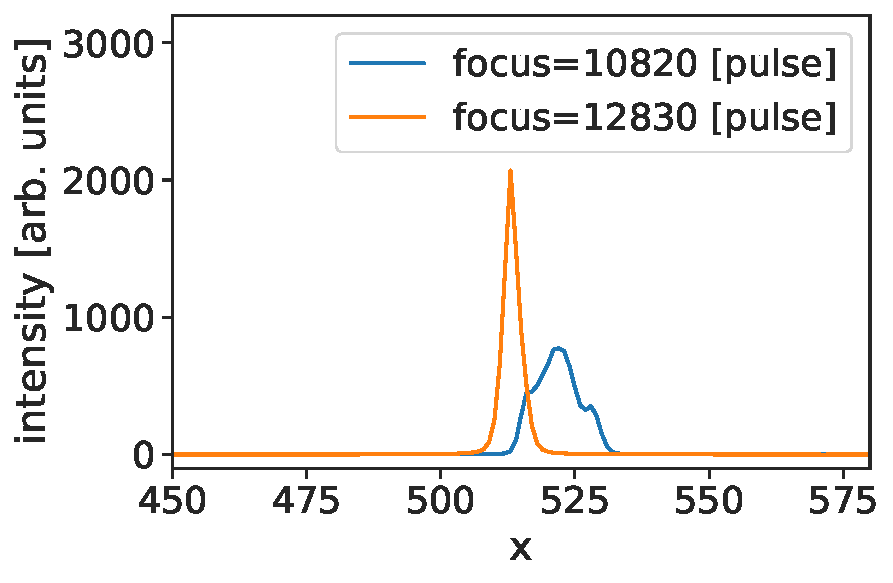
\includegraphics[scale=0.45]{figure/HeNe_focus_example_comparison.pdf}}
    \caption{
    (a)HeNeレーザ光源でのフォーカスパルスの変化とスペクトル幅の関係.オレンジで囲った点は最も焦点が合っているフォーカスパルスが12830のものを示している,
    (b)フォーカスパルスが10820のときと12830のときに得られたスペクトル}
    \label{fig:HeNe_focus_example}
\end{figure}
ここでスペクトル幅は撮影したデータをy軸方向に足し合わせて作成したスペクトル図をガウス関数でフィッティングした際の半値全幅とした.
スペクトル幅が最小値を取る時が焦点が合っている時であるといえる.

% 実際の分光計測で用いるのは焦点があっている時のスペクトルのみである.
% 合焦時のスペクトル幅をより小さくできないかと考え,平面鏡$\mathrm{m_3}$の下に取り付けた一軸手動ステージ及びスリット台の厚さを変更しながらそれぞれで最小スペクトル幅を求めた.
% しかし平面鏡$\mathrm{m_3}$の位置,スリット台の厚さを変えても焦点が合っている時のスペクトル幅は大きくは変わらず,それらの相関関係を見つけることはできなかった.


% % $\pm{1}$次光のスペクトルを観測したとき焦点が合っているフォーカスパルスの値がずれがあった.
% Figure\ \ref{fig:HeNe_focus}(a)にその一例を示す.
% 波長が同じなら色収差による焦点距離の変化は発生しないため,1次光でも-1次光でも関係なくフォーカスの位置は一致するはずである.


% この現象は回折格子に入射する光が平行光でなかった,つまりレンズ$\mathrm{l_1}$とスリット間の距離が焦点距離からずれていたためである.
% 入射光が平行でないということは幅のある入射角で回折格子に入射していると言い換えられる.
% ここで,入射角が$\alpha$から$\alpha+\delta\alpha$までの幅を持っており,入射角$\alpha$,$\alpha+\delta\alpha$に対応する回折角を$\beta$,$\beta+\delta\beta$となるとすると
% \begin{eqnarray}
%     Nm\lambda &=& \mathrm{sin}{\alpha}+\mathrm{sin}{\beta} \\
%     Nm\lambda &=& \mathrm{sin}{(\alpha+\delta\alpha)}+\mathrm{sin}{(\beta+\delta\beta)}
% \end{eqnarray}
% とでき,$\delta\alpha$,$\delta\beta$が微小であるとして$\mathrm{sin}{\delta\alpha}=\delta\alpha,\mathrm{sin}{\delta\beta}=\delta\beta$,$\mathrm{cos}{\delta\alpha}=\mathrm{cos}{\delta\beta}=1$と近似して計算すると,
% \begin{eqnarray}
%     \delta\alpha=-\frac{\mathrm{cos}{\beta}}{\mathrm{cos}{\alpha}}\delta\beta
% \end{eqnarray}
% ここで,$(-\mathrm{cos}{\beta}/\mathrm{cos}{\alpha})$は回折格子の拡大率であり,$\pm{}$1次光で拡大,縮小が反転される.
% したがって,$\delta\alpha$に対応する$\delta\beta$の値は$\pm{}$1次光で異なる.
% これらより回折格子に非平行光が入射したとき,$\pm{}$1次光で回折光の広がり方が異なり,焦点距離が変化する.


% 本研究では回折格子には平行光を当てることを前提に設計していたので,$\pm{1}$次光のスペクトルで焦点の合うフォーカスパルスが一致するように各光学素子を調整した.
% % この際,平面鏡$m_3$の下の一軸手動ステージだけでは光軸方向の変化量が不足していたため,スリットと分光器の筐体の間に3Dプリンタで作成した台を入れることによりさらなる調整を可能にした.
% % スリットの台は厚さ5mmのものから5mmずつ厚くしてゆき最大で厚さ30mmのものまで作成した.
% Figure.\ \ref{fig:HeNe_focus}(b)で平面鏡$m_3$を元の位置から6.5 mm前にし,30 mmの厚さのスリット台を使用して撮影した際の$\pm{1}$次光のスペクトル幅とフォーカスパルスの関係性を示す.
% 図より波長が632.8 nmの時$\pm{1}$次光で焦点が合うフォーカスパルスの値が9500ほどで揃っていることが分かる.
% \floatsetup[figure]{style=plain,subcapbesideposition=top}
% \begin{figure}
%     \sidesubfloat[]{
%         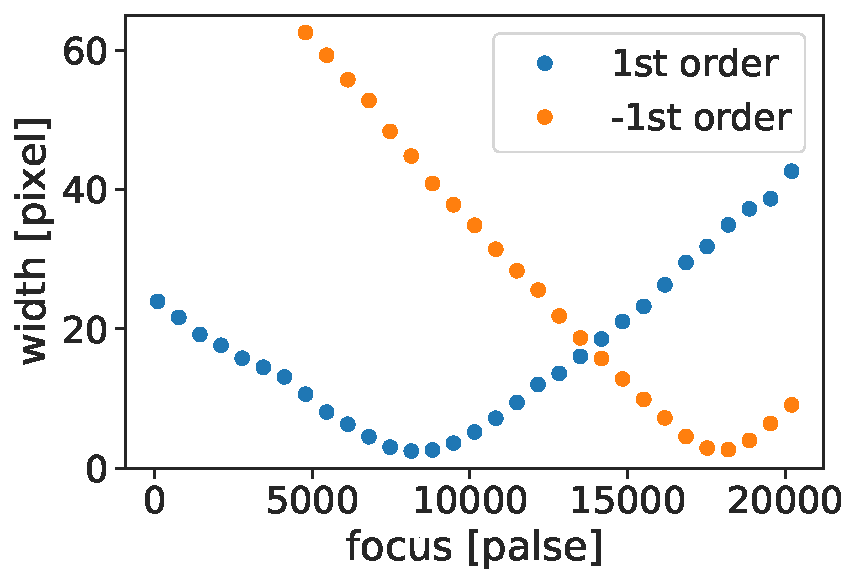
\includegraphics[scale=0.45]{figure/HeNe_focus_before.pdf}}
%     \sidesubfloat[]{
%         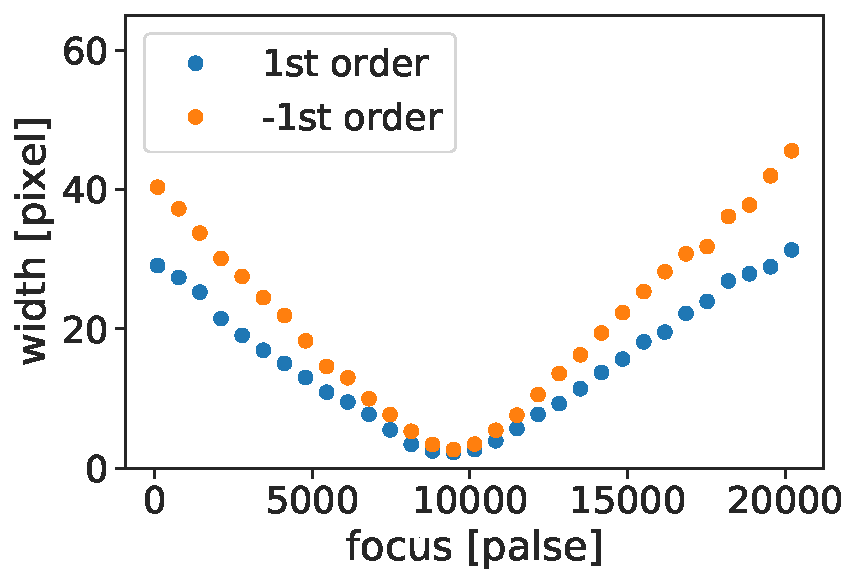
\includegraphics[scale=0.45]{figure/HeNe_focus_after.pdf}}
%     \caption{HeNeレーザを光源にした際の$\pm{1}$次光のスペクトル幅とフォーカスパルスの関係性
%     (a):平面鏡$\mathrm{m_3}$の位置はそのままでスリット台は10mmのものを使用して撮影
%     (b):平面鏡$\mathrm{m_3}$の位置を6.5mm前にしスリット台は30mmのものを使用して撮影}
%     \label{fig:HeNe_focus}
% \end{figure}


% ここから下
本分光器はレンズ$\mathrm{l_1}$とスリット間の距離をレンズの焦点距離にすることで,レンズ$\mathrm{l_1}$に入射する光を平行光にしている.
また同様にレンズ$\mathrm{l_2}$とCCDカメラの受光面の距離をレンズの焦点距離にすることで平行光をレンズ$\mathrm{l_2}$に入射したしたときCCDカメラの受光面に結像されるようにしている.
しかし,レンズ$\mathrm{l_1}$とレンズ$\mathrm{l_2}$をまとめて動かすよう設計しているので平面鏡$\mathrm{m_3}$及びスリットの位置を適切に設定しないと,レンズ$\mathrm{l_1}$とスリットの間の距離,レンズ$\mathrm{l_2}$とCCDカメラ受光面の距離の両方を同時に焦点距離に合わせることはできない.
よってCCDカメラ受光面に焦点が合うように調整されていても,レンズ$\mathrm{l_1}$とスリット間の距離が適切でなく平行光にできていない場合が存在する.
ここで,回折格子に非平行光が入射した際について考える.
入射角が$\alpha$から$\alpha+\delta\alpha$までの幅を持っており,入射角$\alpha$,$\alpha+\delta\alpha$に対応する回折角をそれぞれ$\beta$,$\beta+\delta\beta$となるとすると
\begin{eqnarray}
    Nm\lambda &=& \mathrm{sin}{\alpha}+\mathrm{sin}{\beta} \\
    Nm\lambda &=& \mathrm{sin}{(\alpha+\delta\alpha)}+\mathrm{sin}{(\beta+\delta\beta)}
\end{eqnarray}
とできる.
$\delta\alpha$,$\delta\beta$が微小であるとして$\mathrm{sin}{\delta\alpha}\simeq\delta\alpha,\mathrm{sin}{\delta\beta}\simeq\delta\beta$,$\mathrm{cos}{\delta\alpha}\simeq\mathrm{cos}{\delta\beta}\simeq1$と近似して計算すると,
\begin{eqnarray}
    \delta\alpha\simeq-\frac{\mathrm{cos}{\beta}}{\mathrm{cos}{\alpha}}\delta\beta
\end{eqnarray}
が求められる.
ここで,$-\frac{\mathrm{cos}{\beta}}{\mathrm{cos}{\alpha}}$は回折格子での拡大率であり,本分光器では+1次光で$|\frac{\mathrm{cos}{\beta}}{\mathrm{cos}{\alpha}}|>1$であり像は拡大,-1次光で$|\frac{\mathrm{cos}{\beta}}{\mathrm{cos}{\alpha}}|<1$であり像は縮小する.
$\delta\alpha$に対応する$\delta\beta$の値は$\pm{}$1次光で異なることから,回折格子に非平行光が入射した場合$\pm{}$1次光で回折光の広がり方が異なることになり,結果としてレンズで集光する際の焦点位置が変化する.
平面鏡$\mathrm{m_3}$及びスリットの位置が適切でないと同波長の$\pm{1}$次光のスペクトルを観測する際,CCDカメラ受光面に焦点が合うフォーカスパルスの値にずれが生じる.
図\ \ref{fig:HeNe_focus}(a)にその一例を示す.
これは平面鏡$\mathrm{m_3}$が初期位置で10 mmの厚さのスリット台を使用した際の$\pm{1}$次光におけるフォーカスパルスとスペクトル幅を表している.

回折格子に平行光が入射されるようにするため$\pm{1}$次光のスペクトルで焦点の合うフォーカスパルスが一致するように各光学素子を調整した.
図\ \ref{fig:HeNe_focus}(b)に平面鏡$\mathrm{m_3}$を初期位置から6.5 mm前にし,30 mmの厚さのスリット台を使用して撮影した際の$\pm{1}$次光のフォーカスパルスとスペクトル幅の関係性を示す.
図より波長が632.8 nmの時$\pm{1}$次光で焦点が合うフォーカスパルスの値が9500ほどで揃っていることが分かる.
これによってスリット,及び各平面鏡が正しい位置に配置され,回折格子に平行光が入射されていることが確認できた.
\floatsetup[figure]{style=plain,subcapbesideposition=top}
\begin{figure}
    \sidesubfloat[]{
        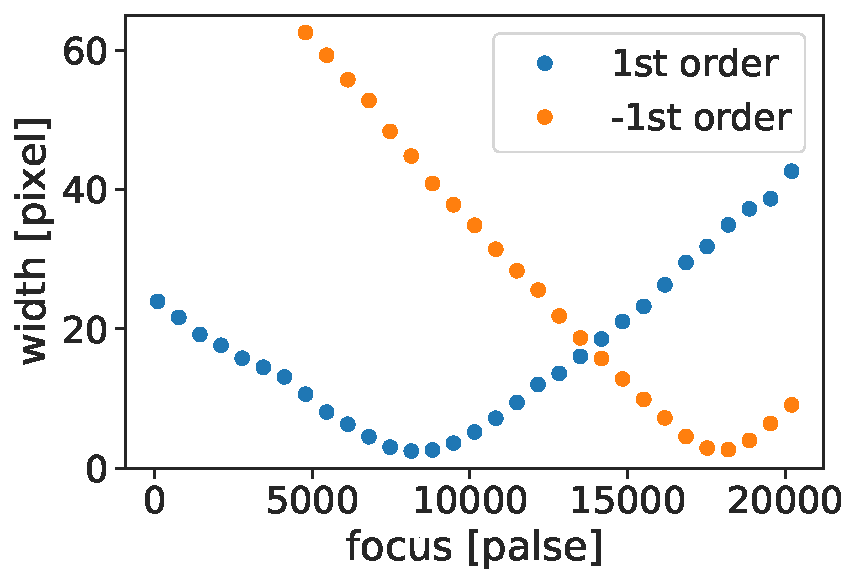
\includegraphics[scale=0.45]{figure/HeNe_focus_before.pdf}}
    \sidesubfloat[]{
        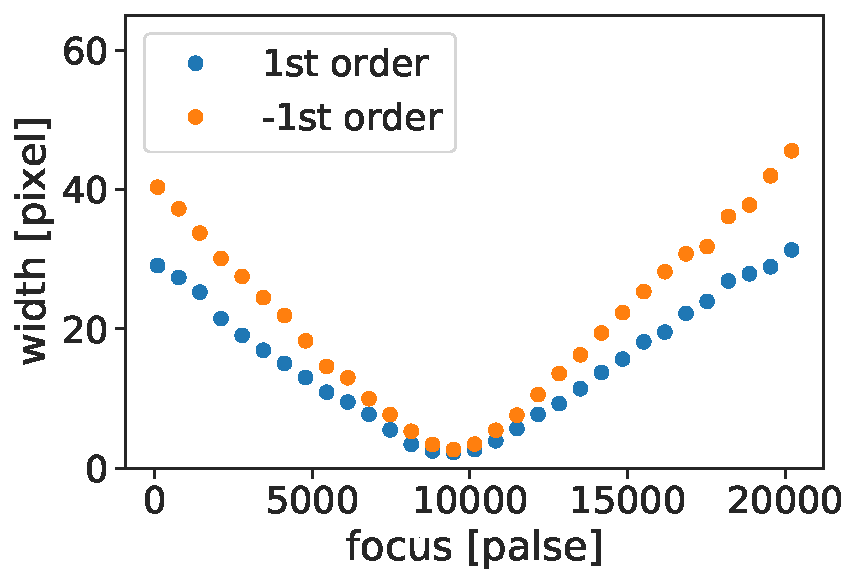
\includegraphics[scale=0.45]{figure/HeNe_focus_after.pdf}}
    \caption{HeNeレーザを光源にした際の$\pm{1}$次光のスペクトル幅とフォーカスパルスの関係性
    (a)平面鏡$\mathrm{m_3}$は初期位置のままで10 mmの厚さのスリット台を使用して撮影,
    (b)平面鏡$\mathrm{m_3}$の位置を初期位置から6.5 mm前にし30 mmの厚さのスリット台を使用して撮影}
    \label{fig:HeNe_focus}
\end{figure}

\subsection{迷光除去}
% 弱いスペクトルを計測しようとしたとき,画面左下側の光の強度が高くなる傾向があることが分かった.
% そのため,目的の波長以外の光が何らかの形でCCDカメラに入ってしまっていると考えた.
図\ \ref{fig:meikou}(a)はスリットに光を入れないで撮影した際のCCDカメラ受光部の光の強度分布である.
図よりCCDカメラの受光部において左下側にわずかに光が当たっていることが分かる.
この光はレンズ下の一軸自動ステージにリミットセンサとして取り付けられているフォトインタラプタによるものである.
このような本来の光路外から発生した光のことを迷光と呼ぶ.
迷光は正確な分光測定を阻害する要因となるため,除去することが望ましい.

CCDカメラに迷光が入らないようにするため,CCDカメラ入口近くに簡易的な遮光壁を光路を遮らないよう設置した(図\ \ref{fig:syakouban}).
\begin{figure}[htbp]
    \centering
    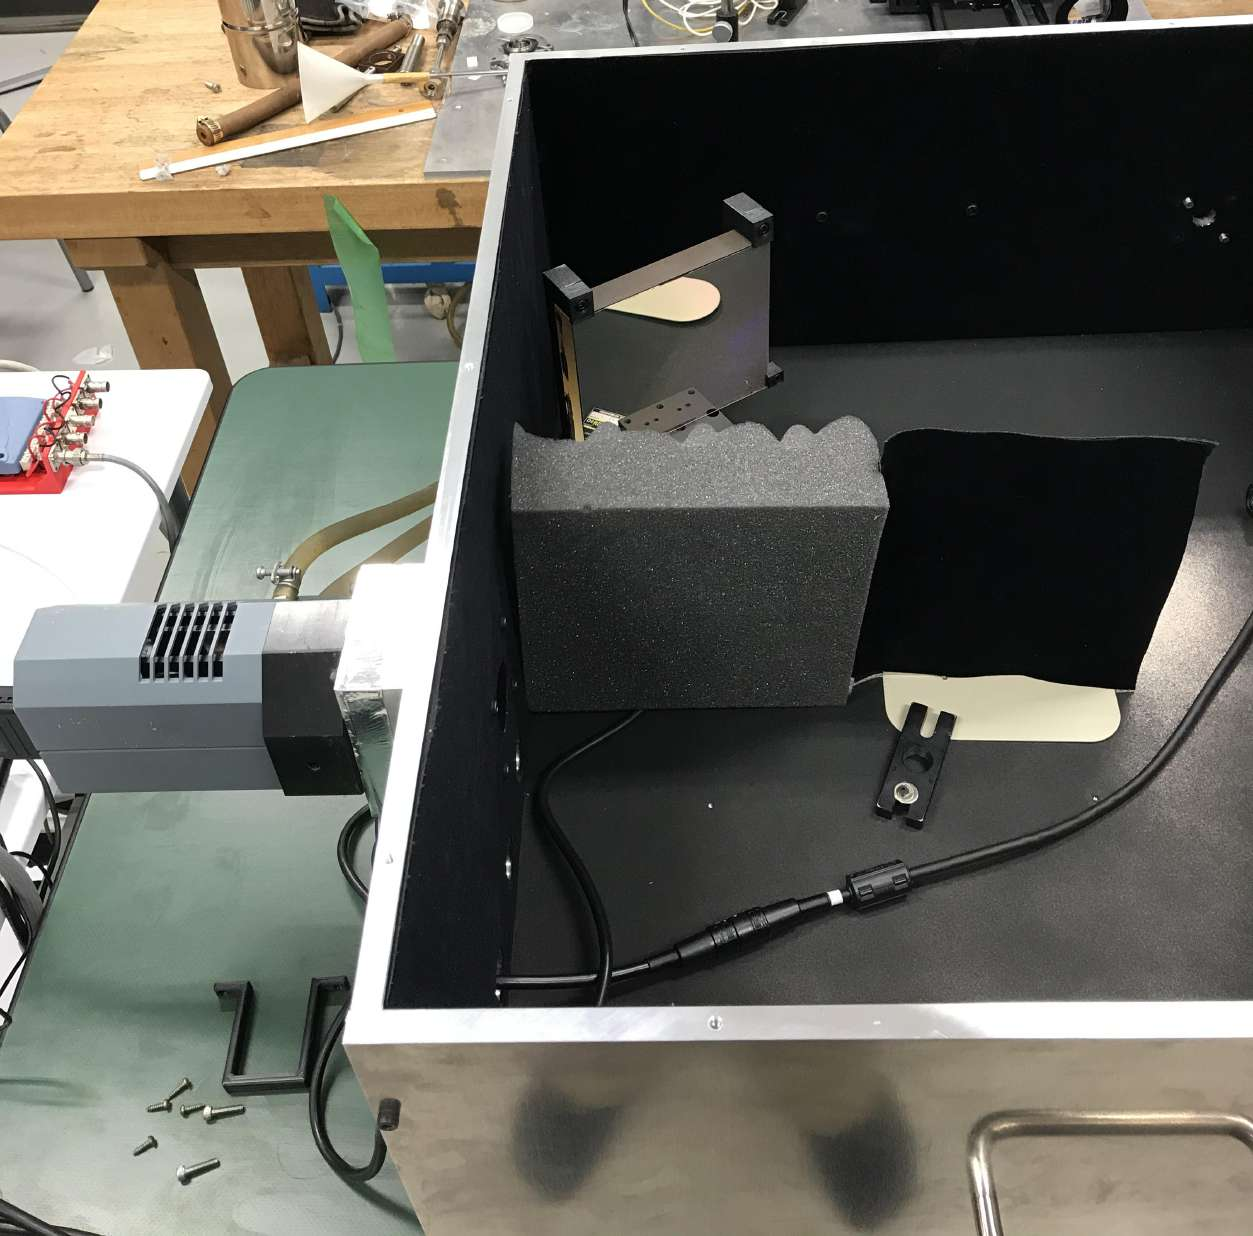
\includegraphics[scale=0.3]{figure/syakouban_compressed.pdf}
     \caption{迷光を遮るために取り付けた簡易的な遮光板}
     \label{fig:syakouban}
\end{figure}
図\ \ref{fig:meikou}(b)は壁を取り付けて再度同じ条件で撮影した際の様子である.
図\ \ref{fig:meikou}(a)と比べて明るさが均一で迷光が除去できていることが分かる.




\floatsetup[figure]{style=plain,subcapbesideposition=top}
\begin{figure}
    \sidesubfloat[]{
        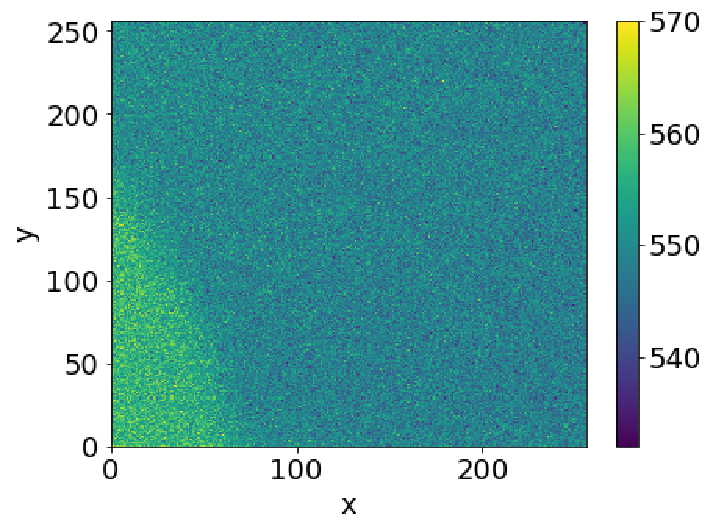
\includegraphics[scale=0.6]{figure/meikou_before.pdf}}
    \sidesubfloat[]{
        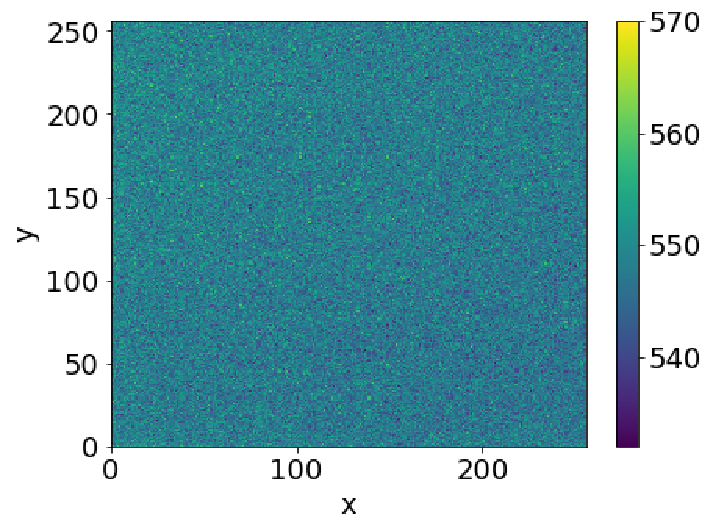
\includegraphics[scale=0.6]{figure/meikou_after.pdf}}
    \caption{遮光板を取り付け前後での迷光の様子.露光時間を1秒,x軸方向,y軸方向ともにビニングサイズを4で撮影した.
    (a)分光器内に遮光壁を取り付ける前に撮影したCCDカメラ受光部の光の強度分布,
    (b)分光器内に遮光壁を取り付けた後に撮影したCCDカメラ受光部の光の強度分布}
    \label{fig:meikou}
\end{figure}



\section{波長校正}
\label{sec:wavelength_calibration}
% 回折格子に入射された光は各波長ごとにx軸方向に分離され,CCDカメラに結像される.
% この際,得られたスペクトルに対応する光の波長は直接求めることはできず,そのスペクトルが得られる回折格子パルスしか分からない.
各スペクトルの波長を求めるためには回折格子パルスと波長の対応関係を求める必要がある.
He原子放電管を用いて$\pm{1}$次光及び0次光の各発光線がCCDカメラの中心部に結像されるような回折格子パルスを記録した.
これを既知のHe原子の各発光線の波長に対してプロットした(図\ \ref{fig:lambda-grating_fitting}).
\begin{figure}[htbp]
    \centering
    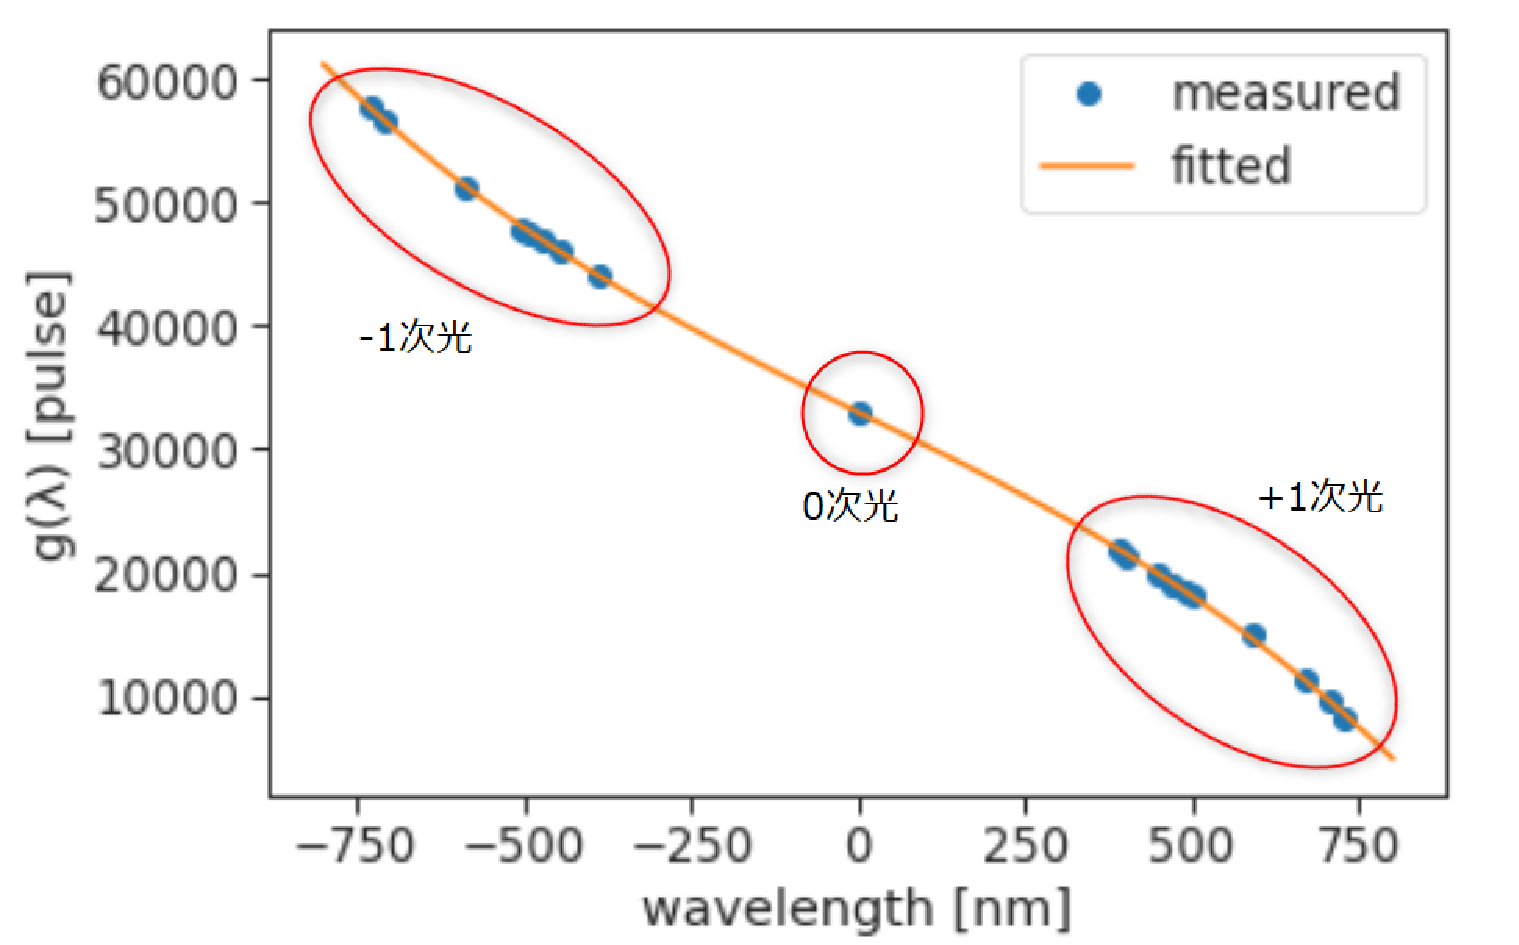
\includegraphics[scale=0.5]{figure/lambda-grating_fitting.pdf}
     \caption{波長と回折格子パルスの対応図.\\
     }
     \label{fig:lambda-grating_fitting}
\end{figure}
今回,グラフを作るために形式的に-1次光で計測したときの波長の値に-1を掛けて表示している.
波長$\lambda$のスペクトルが観測できる回折格子パルスの値$g(\lambda)$を$\lambda$の三次関数
\begin{equation}
     g(\lambda) = a\lambda^3+b\lambda^2+c\lambda+d
\end{equation}
でフィッテイングし,回折格子パルスと波長の対応関係を得た.




\section{色収差補正}
\label{sec:chromatic_aberration_correction}
% レンズを構成物質であるガラスの屈折率は波長によって異なる.
% そのため,レンズの焦点距離は波長によって変化してしまう.
% これを色収差と言い,レンズを使って光を集光させる場合,色収差を補正する必要がある.
単レンズと比べると小さいもののアクロマティックレンズにも色収差は存在する.
そのため,観測したい波長に応じてレンズの位置を調節する必要がある.
波長校正と同じく光源にHe原子放電管を用いて各発光線において図\ \ref{fig:HeNe_focus_example}(a)のような図を作成し,その発光線の波長とそれぞれで一番焦点が合っているフォーカスパルスの値を記録した.
観測波長の関数としてのフォーカスパルス$f(\lambda)$を$\pm{1}$次光それぞれにおいて
\begin{equation}
     f(\lambda) = a+b\lambda^2+c\frac{\lambda^2}{(\lambda^2-d)}
\end{equation}
でフィッテイングした.
図\ \ref{fig:lambda-focus_fitting}(a)(b)に$\pm{1}$次光における波長とフォーカスパルスの対応図を示す.
% これによって,波長とフォーカスパルスの対応関係が得られた.
\floatsetup[figure]{style=plain,subcapbesideposition=top}
\begin{figure}
    \sidesubfloat[]{
        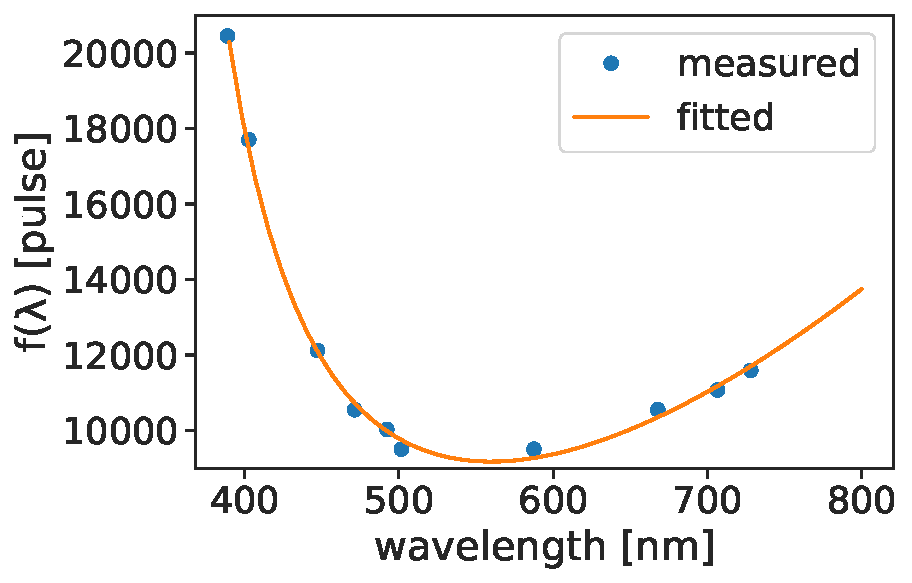
\includegraphics[scale=0.5]{figure/lambda-focus_fitting_1st.pdf}}
    \sidesubfloat[]{
        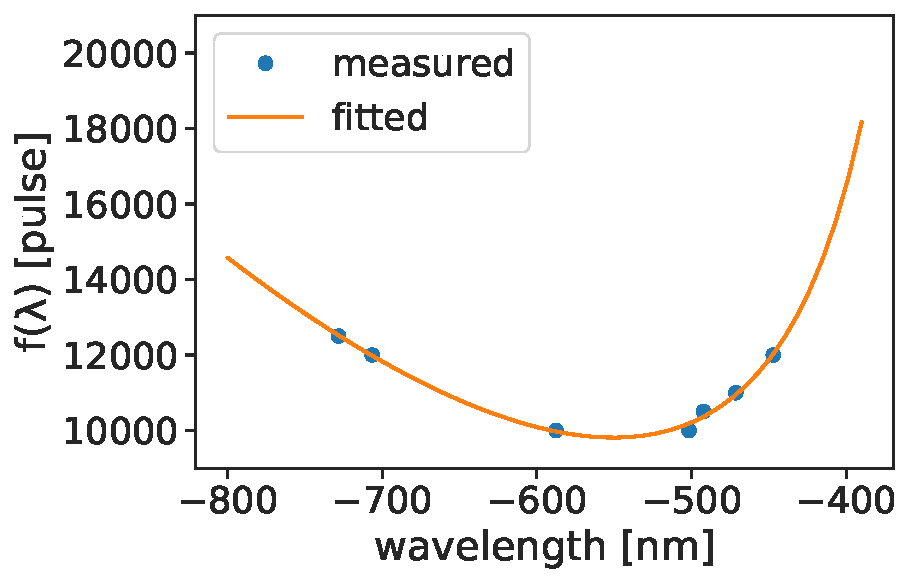
\includegraphics[scale=0.5]{figure/lambda-focus_fitting_-1st.pdf}}
    \caption{波長とフォーカスパルスの対応図\\
    (a)1次光における対応図,
    (b)-1次光における対応図}
    \label{fig:lambda-focus_fitting}
\end{figure}
% また,本実験で使用したアクロマティックレンズ(Edmund Optics TS 大口径アクロマティックレンズ 102 × 1525 枠付き)の色収差は性能データよりFig.\ \ref{fig:focal_shift_lense}のようになっている.
% \begin{figure}[htbp]
    % \centering
    % 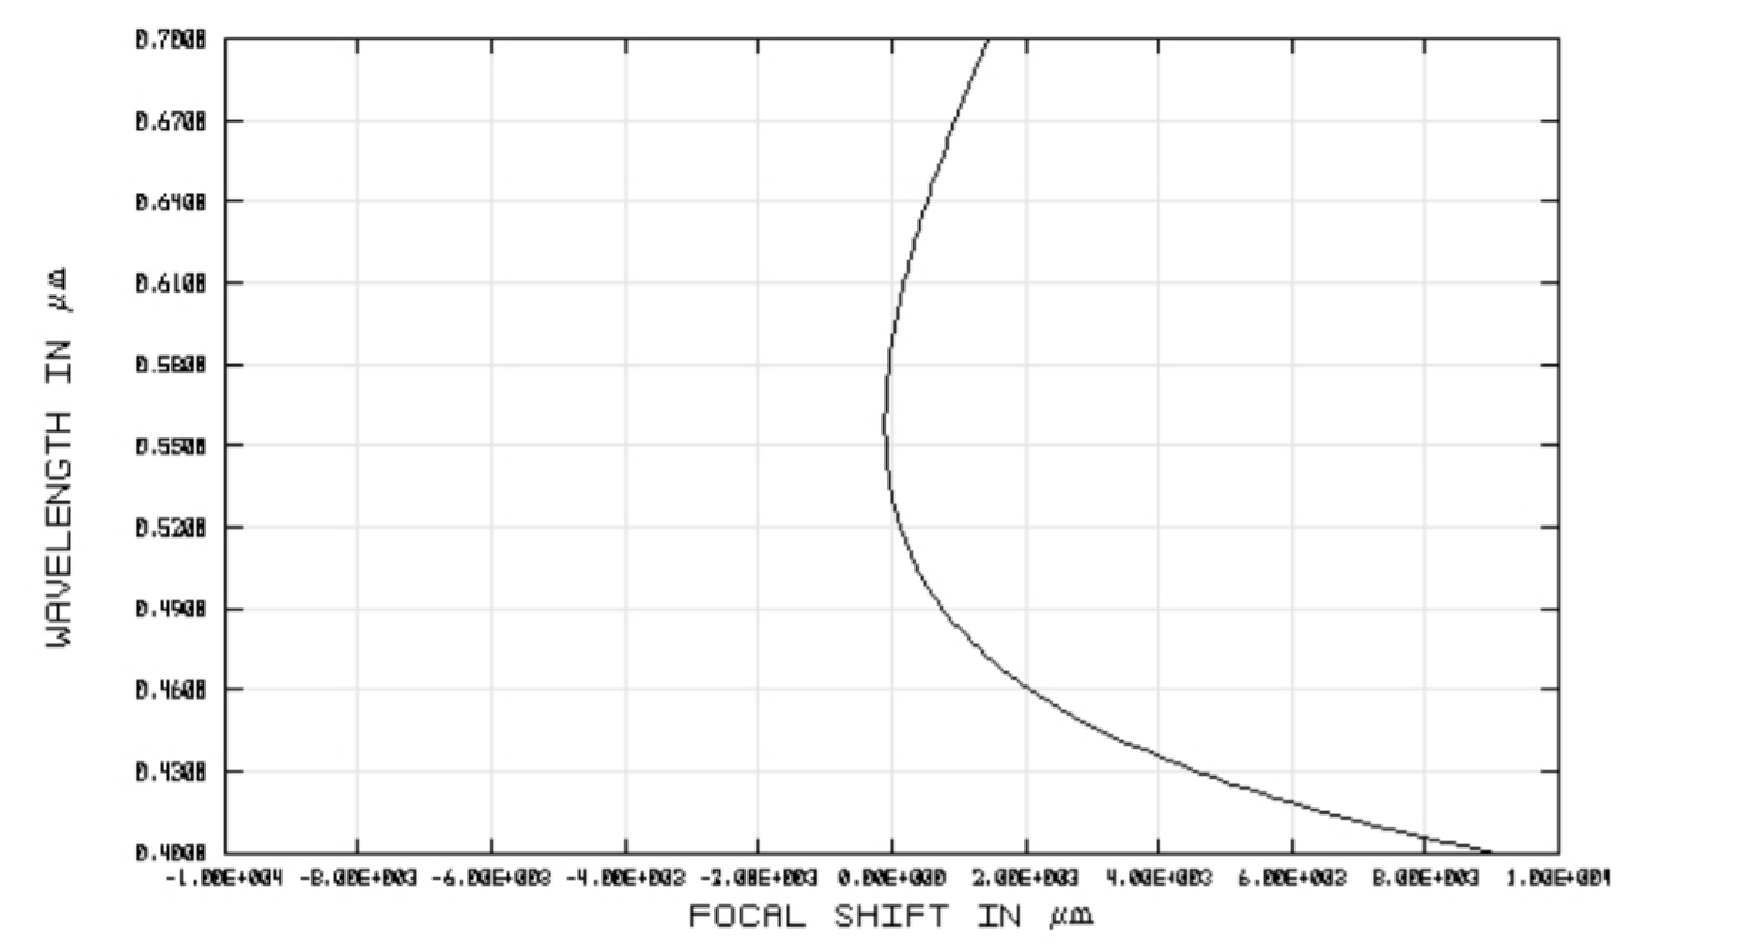
\includegraphics[scale=0.5]{figure/focal_shift_lense.pdf}
    % \caption{使用レンズの波長ごとの焦点シフト}
    % \label{fig:focal_shift_lense}
% \end{figure}
% Fig.\ \ref{fig:lambda-focus_fitting}ではレンズの設計通りの波長と焦点距離の関係を求めることができていると分かる.

前セクションの波長校正と合わせて,波長,回折格子パルス,フォーカスパルスの対応関係を得た.
これによって,欲しい波長範囲を指定することで回折格子パルス,フォーカスパルスが決定し制御できるようになった.
実際の実験ではPythonスクリプトによって自動回転ステージ,一軸自動ステージ及びCCDカメラの制御を行っている.
% ()に自動回転ステージ,一軸自動ステージの制御を行っているスクリプトの一例を示す.
\chapter{実験}
\label{chap:evaluation}

% \section{装置幅}
% 分光器に単波長の光を入射させたとしても,スペクトルは収差やスリット幅に依存した有限の幅を持つ.
% この各分光器ごとに固有であるスペクトルの幅を装置幅と呼ぶ.
% ここではスペクトル形状をガウス関数でフィッティングした際の半値全幅を装置幅と定義する.
\section{実験概要}
% Fe-Neホローカソードランプを光源に波長範囲約400 nm~730 nmで対応する回折格子パルスを変えながら150個のデータを撮影した.
Fe-Neホローカソードランプを光源に回折格子パルスを8000から90ずつ大きくしていき21410まで変えながら150個のデータを撮影した.
これは波長範囲で約400~730 nmに対応する.
露光時間は3秒,y軸方向のビニングサイズを4に設定した.
配置したホローカソードランプとスリットの外観写真を図\ \ref{fig:lamp_slit}に示す.
\begin{figure}[htbp]
    \centering
    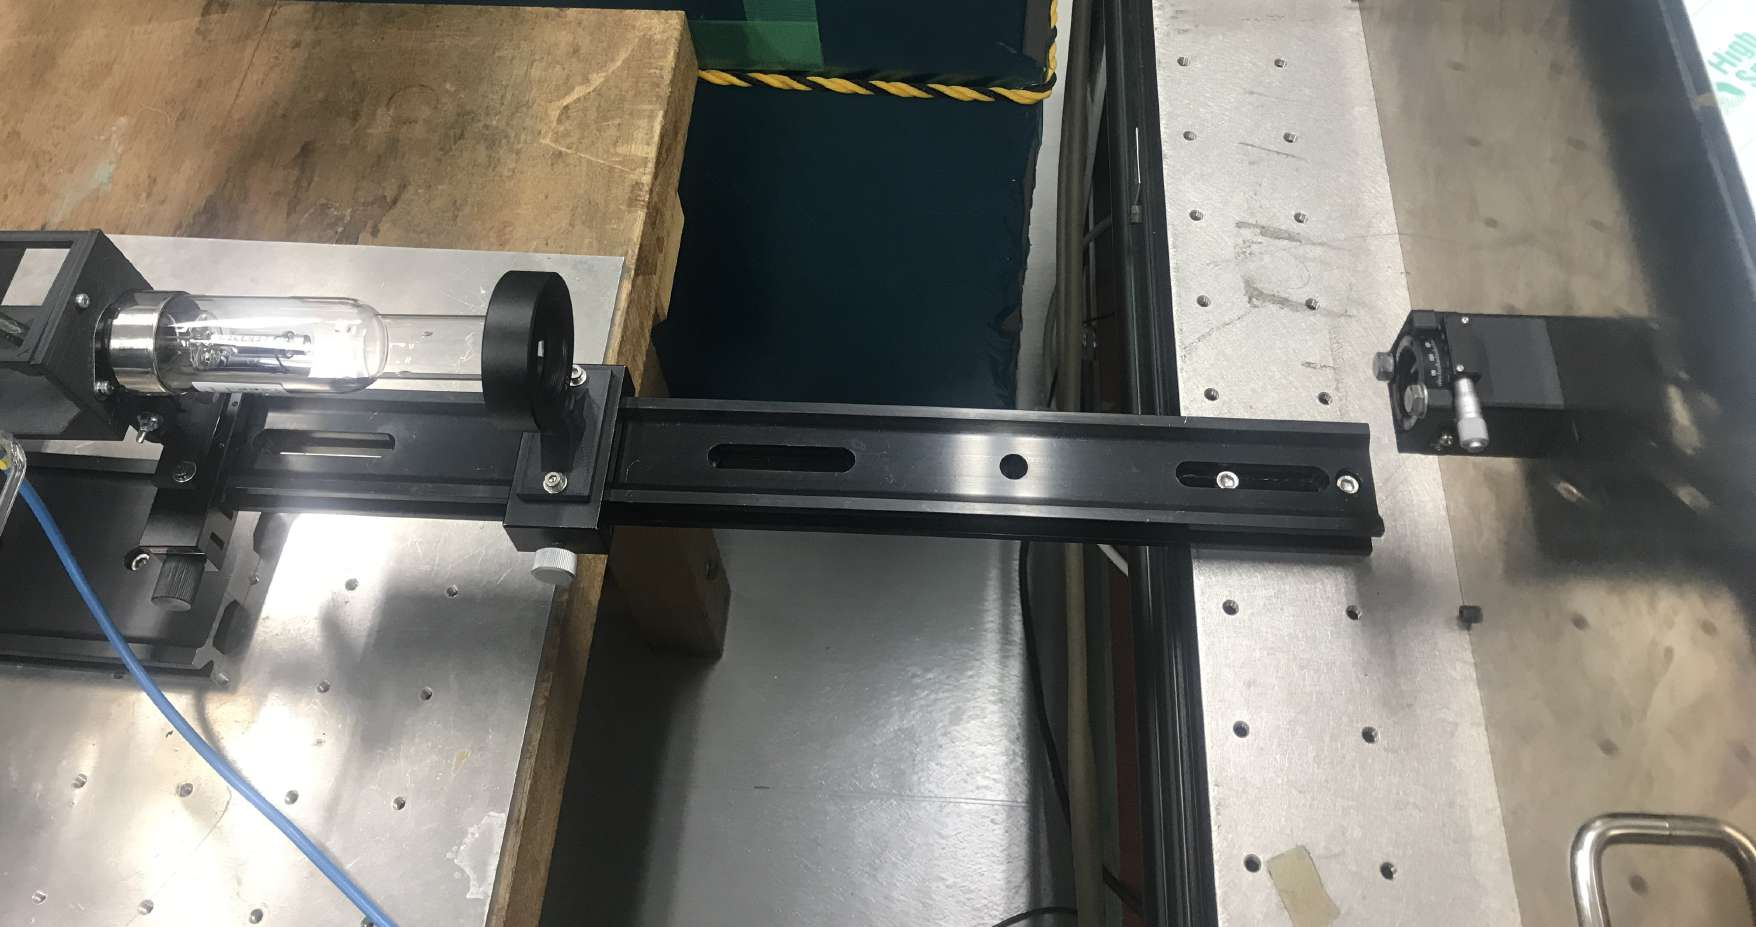
\includegraphics[scale=0.3]{figure/lamp_slit_compressed.pdf}
    \caption{Fe-Neホローカソードランプとスリットの配置の外観図}
    \label{fig:lamp_slit}
\end{figure}


ここで撮影した計測データの例として図\ \ref{fig:spectrum_example}に中心波長521.5 nmにおいて撮影されたCCDカメラ受光部の光の強度分布図を示す.
\begin{figure}[htbp]
    \centering
    \includegraphics[scale=1]{figure/spectrum_example.pdf}
    \caption{光源にFe-Neランプを用いて撮影した中心波長521.5 nmのCCDカメラ受光部の二次元光強度分布}
    \label{fig:spectrum_example}
\end{figure}
また図\ \ref{fig:spectrum_example2}は図\ \ref{fig:spectrum_example}の輝線部分(図\ \ref{fig:spectrum_example}におけるy軸方向に115~160ピクセル部分)の各ピクセルをy軸方向に平均しプロットした図である.
ここで縦軸は光の強度を表す.
\begin{figure}[htbp]
    \centering
    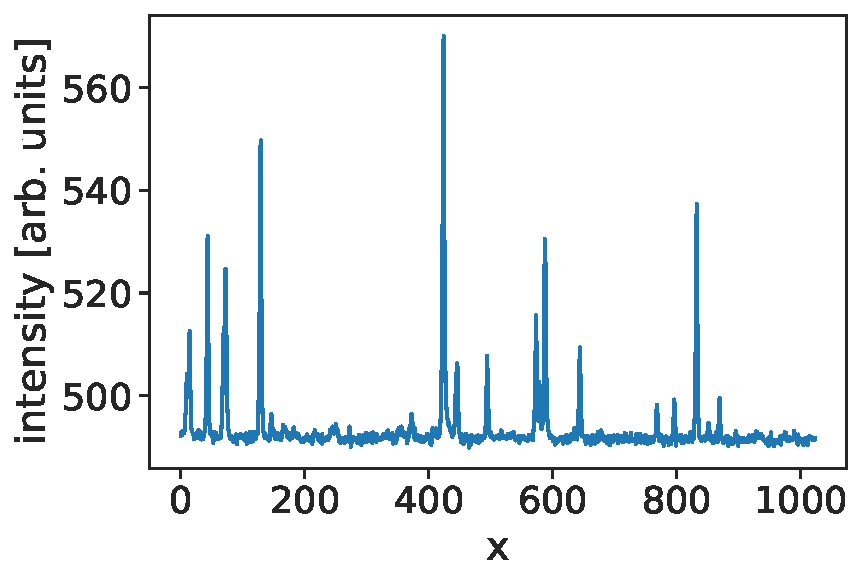
\includegraphics[scale=0.8]{figure/spectrum_example2.pdf}
    \caption{中心波長521.5 nmにおいて撮影したFeのスペクトル}
    \label{fig:spectrum_example2}
\end{figure}
撮影した150枚全てで図\ \ref{fig:spectrum_example2}のようなスペクトルを作成した.

\section{スペクトルの結合}
150枚のデータを撮影した際それぞれの隣り合うデータは一部が共通の波長領域になるように設定している.
そのため,150枚のスペクトル図は波長方向に一部を重ねて結合することができる.
ここで例として中心波長518.9 nmにおけるスペクトルと中心波長516.4 nmにおけるスペクトルを図\ \ref{fig:spectrum_example105},図\ \ref{fig:spectrum_example106}に示す.
\begin{figure}[htbp]
    \centering
    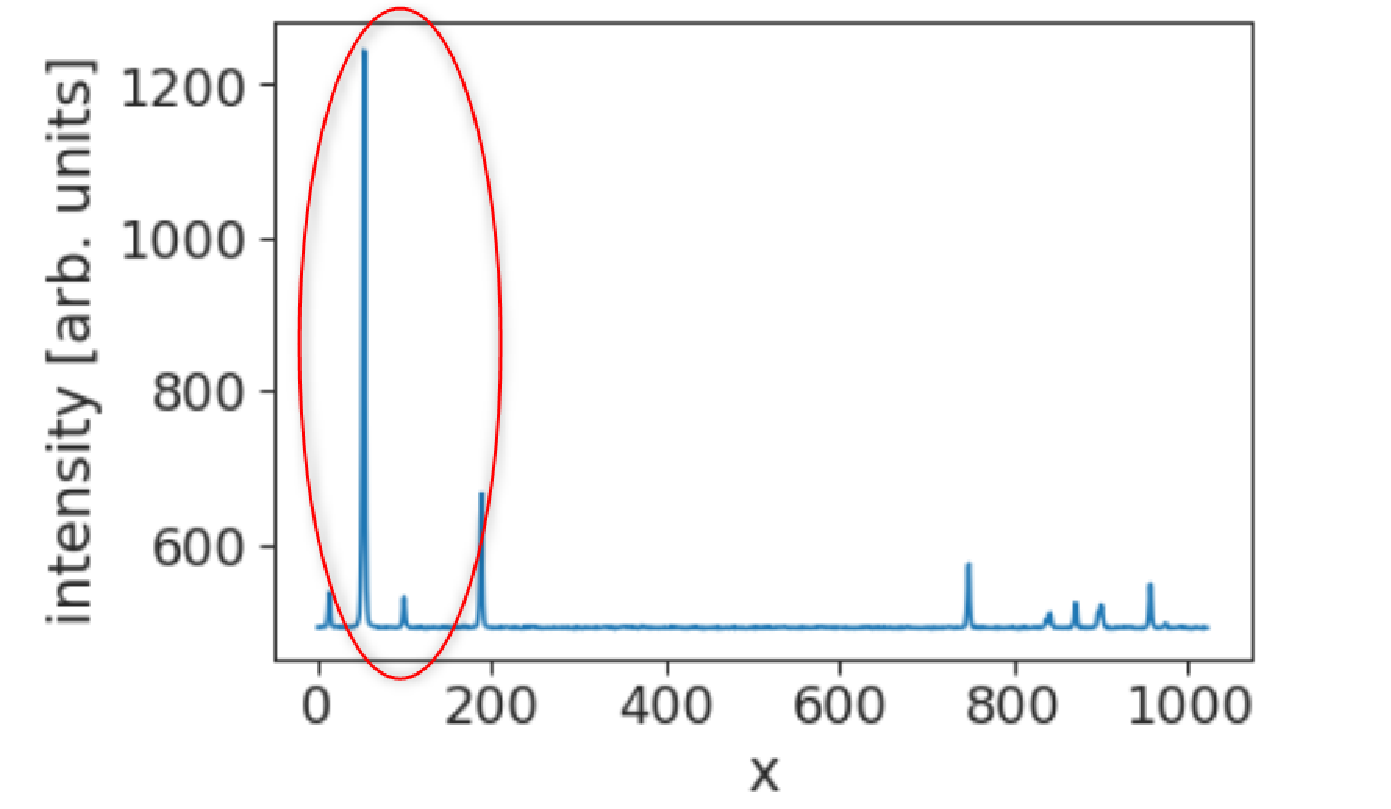
\includegraphics[scale=0.6]{figure/spectrum_example_105.pdf}
    \caption{中心波長518.9 nmにおけるスペクトル.赤く囲った部分が中心波長516.4 nmにおけるスペクトルと共通している.}
    \label{fig:spectrum_example105}
\end{figure}
\begin{figure}[htbp]
    \centering
    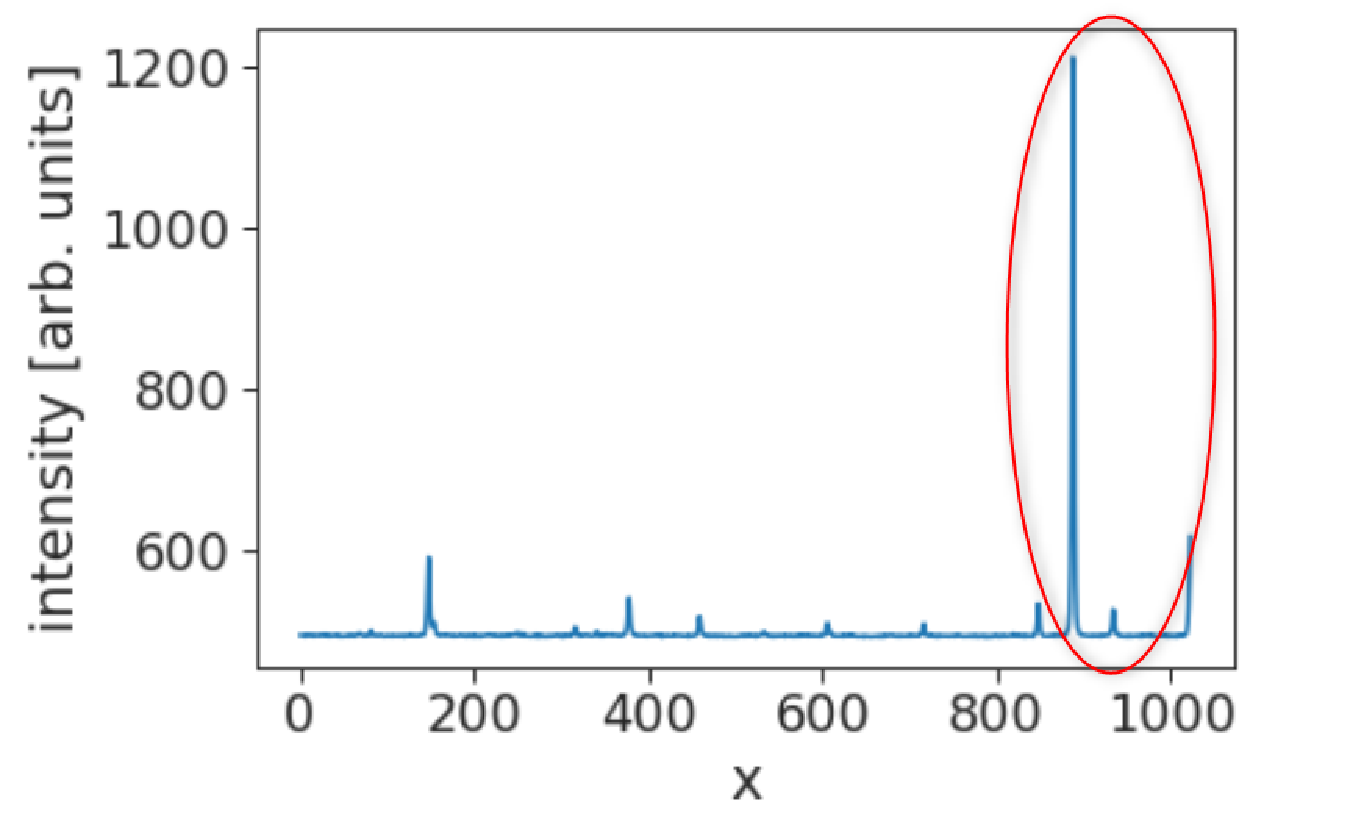
\includegraphics[scale=0.6]{figure/spectrum_example_106.pdf}
    \caption{中心波長516.4 nmにおけるスペクトル.赤く囲った部分が中心波長518.9 nmにおけるスペクトルと共通している.}
    \label{fig:spectrum_example106}
\end{figure}
赤線で囲まれた部分のスペクトルの形が一致していることからこの部分で同じ波長領域を観測していることが分かる.
重なり幅を調べるため相関係数を用いる.
中心波長518.9 nmにおけるスペクトルと中心波長516.4 nmにおけるスペクトルを$d$ピクセルだけ重ねた際の重なり部分における相関係数$r$を求め,$r$が1に最も近くなる$d$を調べた.
相関係数は以下の式で求められる.
\begin{equation}
     r = \frac{\frac{1}{d}\sum_{i=1}^{d} {(X_i-\overline{X})(Y_{1024-i+1}-\overline{Y})}}{{\sqrt{\frac{1}{d}\sum_{i=1}^{d} {(X_i-\overline{X})^2}}\times\sqrt{{\frac{1}{d}\sum_{i=1}^{d} {(Y_{1024-i+1}-\overline{Y})^2}}}}}
\end{equation}
ここで$\overline{X}$,$\overline{Y}$はそれぞれ$X$,$Y$の平均値である.
今回$X$は中心波長518.9 nmにおけるスペクトルの光の強度を,$Y$は中心波長516.4 nmにおけるスペクトルの光の強度を表す.
重なり幅$d$を変化させたときの相関係数$r$の変化の様子を図\ \ref{fig:correlation_coefficients}に示す.
\begin{figure}[htbp]
    \centering
    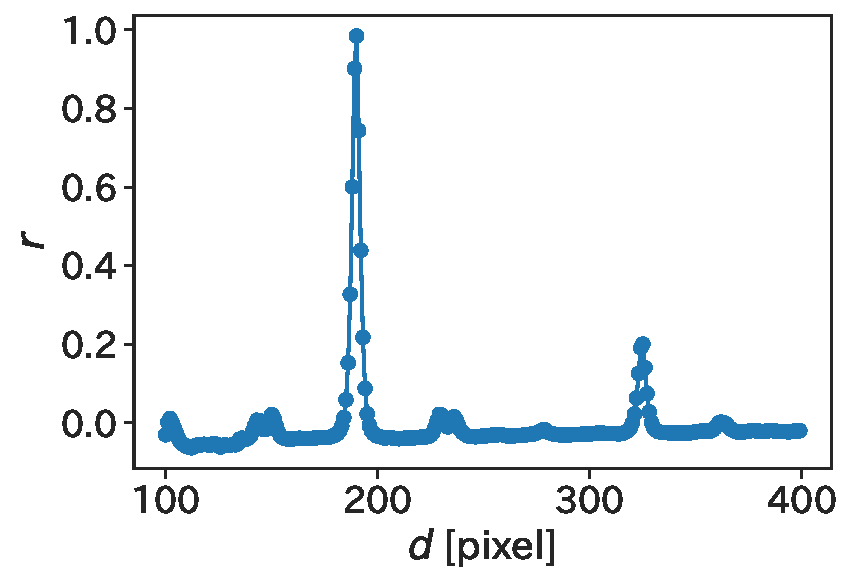
\includegraphics[scale=0.7]{figure/correlation_coefficients.pdf}
    \caption{重なり幅dを変化させたときの中心波長518.9 nmにおけるスペクトルと中心波長516.4 nmにおけるスペクトルの相関関数の変化}
    \label{fig:correlation_coefficients}
\end{figure}
図\ \ref{fig:correlation_coefficients}より中心波長518.9 nmにおけるスペクトルと中心波長516.4 nmにおけるスペクトルは190ピクセル分だけ重ねられることが分かった.
同様のことを他のスペクトルに対しても行い重なり幅を求め,全てのスペクトルを波長方向に結合した.

\section{波長校正}
4.3節の波長校正より150枚の各スペクトルの中心の波長を求めることができるが,これだけではそれぞれのピクセルにあるスペクトルの波長を求めることはできない.
ここで重ね合わせる前の各スペクトルの中心の波長を求め,線形補完することで各ピクセルの波長を求めた.
$n$枚目のスペクトルの$x=a$の波長($\lambda_{n,a}$)を表す式を以下に示す.
\begin{equation}
     \lambda_{n,a} = \lambda_n + \frac{(a-512)(\lambda_n-\lambda_{n+1})}{1024-d_n} 
\end{equation}
ここで$\lambda_n$は$n$枚目のスペクトルの中心波長,$d_n$は$n$枚目と$n+1$枚目のスペクトルの重なり幅を表す.
右辺第二項の分母$(1024-d_n)$は$n$枚目のスペクトルと$n+1$枚目のスペクトルを重ね合わせた時のそれぞれのスペクトルの中心間距離を表す.
$(a-512)$は$n$枚目のスペクトルにおける中心ピクセル$(x=512)$との距離を表す.
これによりスペクトルの横軸を波長に変換した.
150枚のスペクトルを結合させ,横軸を波長に変換した図が図\ \ref{fig:fe_wide_range}である.
\begin{figure}[htbp]
    \centering
    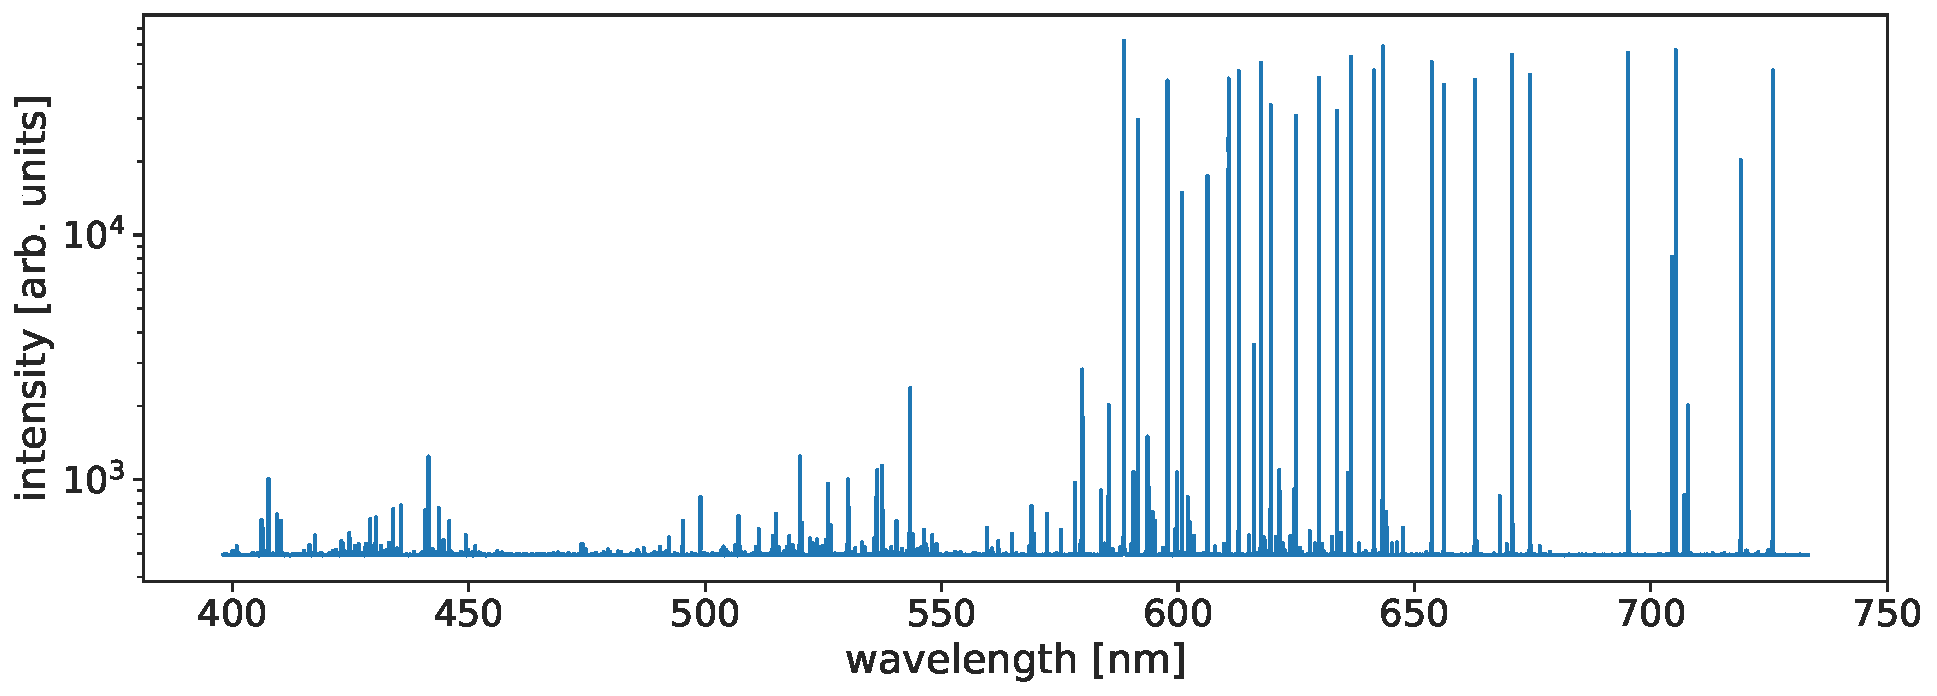
\includegraphics[scale=0.5]{figure/fe_wide_range.pdf}
    \caption{撮影した波長範囲でのFeのスペクトル(縦軸は対数目盛)}
    \label{fig:fe_wide_range}
\end{figure}
% また,Fig.\ \ref{fig:fe_wide_range}の光が低強度の部分を拡大したものがFig.\ \ref{fig:fe_wide_range_zoom}である.
% \begin{figure}[htbp]
    % \centering
    % 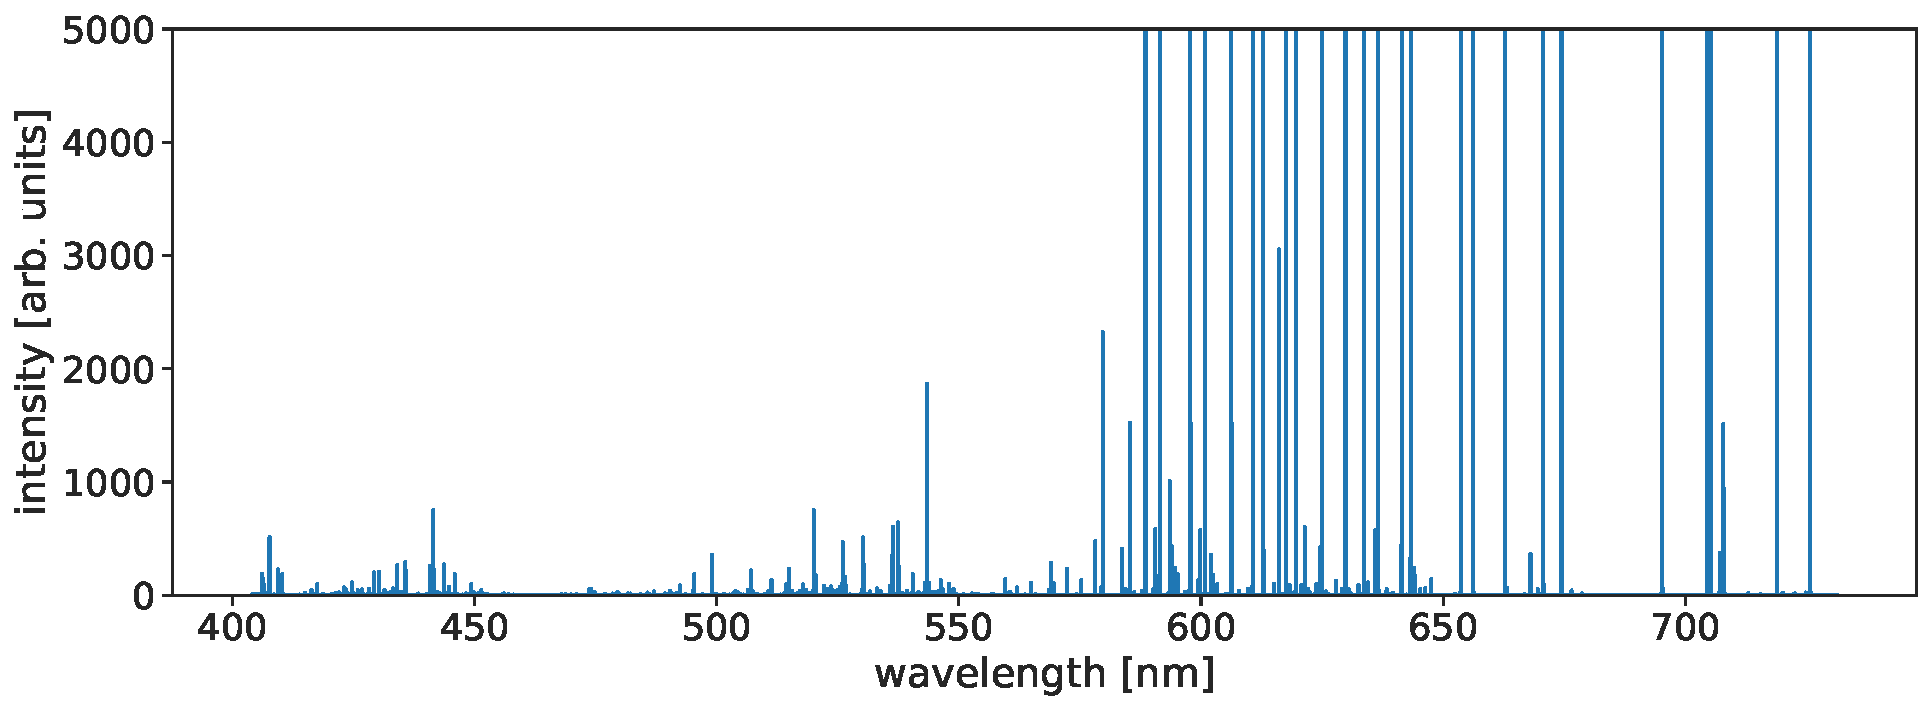
\includegraphics[scale=0.5]{figure/fe_wide_range_zoom.pdf}
    % \caption{Fig.\ \ref{fig:fe_wide_range}の光強度が小さい部分の拡大図}
    % \label{fig:fe_wide_range_zoom}
% \end{figure}
% 本研究で使用しているCCDカメラの情報処理容量は16bitであるため,各ピクセルにおいて$2^{16}-1=65535$までしか光の強度を表すことができない.
% Fig.\ \ref{fig:fe_wide_range}を見ると高波長側で強度が大きいスペクトルが存在する.

\section{装置幅}
% 分光器に単波長の光を入射させたとしても,スペクトルは収差やスリット幅に依存した有限の幅を持つ.
% この各分光器ごとに固有であるスペクトルの幅を装置幅と呼ぶ.
分光器に単色光を入射したときに得られるスペクトルをガウス関数でフィッティングした際の半値全幅を装置幅と定義する.
先ほど実験で用いたFe-Neホローカソードランプは装置幅以外の要因でのスペクトルの広がりは小さい.
そのため,本研究ではFeのスペクトルをガウス関数でフィッティングした際の半値全幅を装置幅とする.

本研究で使用しているCCDカメラは各ピクセルにおいて$2^{16}-1=65535$までしか光の強度を表すことができない.
飽和したピクセルは光の強度を正しく表すことができず,そのピクセルから作成されるスペクトルは正確な幅を求めることができない.
そこで今回は光の強度が50000以下のスペクトルを用いて装置幅を求める.
% ここで,Fig.\ \ref{fig:fe_wide_range}において強度の大きいスペクトルは飽和して信号電荷が上限値となっているピクセルを含んでいる可能性がある.
% このようなピクセルを使ってスペクトル図を作成すると幅を求める際に正確性が失われる.
% そのため,この強度の高いスペクトルはFeによる発光線ではなく封入ガスであるNeによる発光線を含んでいると考えた.
% 今回,装置幅を求めるために欲しいのはFeのスペクトルでありNeのスペクトルは不要である.
% また,装置幅を求めるためにはFig.\ \ref{fig:spectrum_example2}にあるほど多数のスペクトルは必要としておらず,S/N比の大きいスペクトルが全体で数十個あれば十分である.
% そこでFig.\ \ref{fig:fe_wide_range}に無数にあるピークの中から,装置幅を求めるのに使用するピークを抽出した.
% そのため,Fig.\ \ref{fig:fe_wide_range}のスペクトルから光の強度が150から40000のピークをピックアップし,これらを用いて装置幅を求めることとする.
装置幅を求めるのに使用するピークを抽出するためにPythonのパッケージであるscipyのfind\_peaks関数\cite{scipy}を用いた.
find\_peaks関数は高さなどの特性を指定して極大値を見つけ出す関数である.
装置幅を求めるために,図\ \ref{fig:fe_wide_range}のスペクトルから光の強度が200から50000のピークを抽出した.
抽出したピークを図\ \ref{fig:fe_wide_range_peak}に示す.
\begin{figure}[htbp]
    \centering
    \includegraphics[scale=0.5]{figure/fe_wide_range_peak.pdf}
    \caption{装置幅を求めるために抽出したピーク点(赤丸)}
    \label{fig:fe_wide_range_peak}
\end{figure}
図\ \ref{fig:fe_wide_range_peak}の赤点をピークに持つスペクトルをそれぞれガウス関数でフィッティングし,半値全幅を求めた.
% Fig.\ \ref{fig:instrumental_function}は各スペクトルの半値全幅を波長に対してプロットしたものである.
% \begin{figure}[htbp]
%     \centering
%     \includegraphics[scale=0.7]{figure/instrumental_function.pdf}
%     \caption{分光器装置幅の波長依存性}
%     \label{fig:instrumental_function}
% \end{figure}

\section{理論装置幅との比較}
図\ \ref{fig:instrumental_function_design}上に求めたスペクトルの半値全幅をプロットした(図\ \ref{fig:instrumental_function2}).
\begin{figure}[htbp]
    \centering
    \includegraphics[scale=0.7]{figure/instrumental_function2.pdf}
    \caption{分光器装置幅と各条件での理論装置幅の比較}
    \label{fig:instrumental_function2}
\end{figure}
レンズの収差や回折限界による影響を受けないと仮定すると理論装置幅は3.0 pmほどになるが,実際の装置幅は波長に依存なく6.9~9.1 pmに分布していた.

% レンズが本来の性能通りに集光できていれば3.0 pmの装置幅は実現できるはずである.
% しかし,今回の測定ではレンズは理想通りにCCDカメラに対して結像できなかったため装置幅が大きくなってしまった.
レンズの集光性能が十分であるため理論装置幅を実現できると考えていたが,今回の計測において分光器は理論装置幅を実現することができなかった.
これは他の要因の影響を受けているためだと考えられるが,その要因についてはまだ判明しておらず今後の課題である.
% \include{result}
\chapter{結言}
コリメータ及び結像器にレンズを用いて光学系を共軸に配置した分光器を製作した.
測定波長,回折格子の角度,検出器受光面に焦点が合うレンズの位置の対応関係を求め,レンズの色収差を補正した.
また,これらの対応関係を用いてPythonスクリプトによって制御を自動化した.
スポット解析によって求めた使用レンズの設計上の結像の大きさ,回折限界,スリット幅などから求まる装置幅の理論値を計算したところ,3.0 pmほどとなった.
Fe-Neホローカソードランプを光源に用いた測定を行い,分光器の装置幅を求めた.
装置幅は波長に依存なく6.9~9.1 pmに分布していた.

\label{chap:conclusion}
\chapter*{謝辞}
本研究を行うにあたり,蓮尾昌裕教授,四竈泰一准教授,Arseniy Kuzmin講師,藤井恵介助教には様々なご指導をしていただきました.特に藤井助教には日々の研究活動の方針をはじめ本論文の執筆に至るまで丁寧にご指導いただき,大変お世話になりました.また,同期の友人たちとはゼミなど通じ様々な意見を交わし理解を深めることができました.お世話になった皆様に深くお礼申し上げます.


%% reference
\renewcommand\refname{\vskip -1cm}
% \footnotesize
\bibliographystyle{junsrt}
\bibliography{refs}



% \begin{figure}[htbp]
    \centering
    \includegraphics[scale=1]{figure/grating.png}
    \caption{回折格子における光の回折}
\end{figure}
% https://dl.cdn-anritsu.com/ja-jp/test-measurement/files/Technical-Notes/White-Paper/MS9740A_JR1100.pdf

\begin{figure}[htbp]
    \centering
    \includegraphics[scale=1]{figure/achromaticlense.png}
    \caption{アクロマティックレンズでの色収差の補正}
\end{figure}
% http://www.mekatoro.net/digianaecatalog/chuo-sougou/book/chuo-sougou-P0904.pdf


\begin{figure}[htbp]
    \centering
    \includegraphics[scale=0.8]{figure/spectrometer_design.png}
    \caption{分光器概略図}
\end{figure}


\floatsetup[figure]{style=plain,subcapbesideposition=top}
\begin{figure}
    \sidesubfloat[]{
        \includegraphics[scale=0.7]{figure/lense_system.png}}
    \sidesubfloat[]{
        \includegraphics[scale=0.7]{figure/grating_system.png}}
    \caption{.
    (a):レンズ周りの部品構成
    (b):回折格子周りの部品構成}
\end{figure}

\floatsetup[figure]{style=plain,subcapbesideposition=top}
\begin{figure}
    \sidesubfloat[]{
        \includegraphics[scale=0.5]{figure/HeNe_focus_before.png}}
    \sidesubfloat[]{
        \includegraphics[scale=0.5]{figure/HeNe_focus_after.png}}
    \caption{HeNeレーザを光源にした際の$\pm{1}$次光のスペクトル幅とフォーカスパルスの関係性
    (a):平面鏡$m_3$の位置はそのままでスリット台は10mmのものを使用して撮影
    (b):平面鏡$m_3$の位置を6.5mm前にしスリット台は30mmのものを使用して撮影}
\end{figure}


\floatsetup[figure]{style=plain,subcapbesideposition=top}
\begin{figure}
    \sidesubfloat[]{
        \includegraphics[scale=0.5]{figure/meikou_before.png}}
    \sidesubfloat[]{
        \includegraphics[scale=0.5]{figure/meikou_after.png}}
    \caption{スリットに光を入れないで撮影した際の強度分布.露光時間は1秒,x軸方向,y軸方向ともにビニングサイズを4とした.
    (a):分光器内に壁を取り付ける前に撮影したもの
    (b):分光器内に壁を取り付けた後に撮影したもの}
\end{figure}


\begin{figure}[htbp]
    \centering
    \includegraphics[scale=1]{figure/lambda-grating_fitting.png}
    \caption{波長と回折格子パルスの対応図}
\end{figure}


\floatsetup[figure]{style=plain,subcapbesideposition=top}
\begin{figure}
    \sidesubfloat[]{
        \includegraphics[scale=0.5]{figure/lambda-focus_fitting_1st.png}}
    \sidesubfloat[]{
        \includegraphics[scale=0.5]{figure/lambda-focus_fitting_-1st.png}}
    \caption{波長とフォーカスパルスの対応図\\
    (a):1次光のフィッテイング結果
    (b):-1次光のフィッテイング結果}
\end{figure}

\begin{figure}[htbp]
    \centering
    \includegraphics[scale=1]{figure/spectrum_example.png}
    \caption{光源をFeランプで撮影した波長520nm付近の光の二次元強度分布}
\end{figure}

\begin{figure}[htbp]
    \centering
    \includegraphics[scale=1]{figure/spectrum_example2.png}
    \caption{光源をFeランプで撮影した波長520nm付近のスペクトル}
\end{figure}

\begin{figure}[htbp]
    \centering
    \includegraphics[scale=0.5]{figure/fe_wide_range.png}
    \caption{光源をFeランプで撮影した測定波長範囲でのスペクトル}
\end{figure}





\end{document}
